\documentclass{article}
\usepackage{graphicx} % Required for inserting images
\usepackage{listings} % Replacing minted with listings
\usepackage[margin=25mm]{geometry}
\usepackage[indent=0mm]{parskip}
\usepackage{braket}
\usepackage[math]{cellspace}
\usepackage{xcolor} % to access the named colour LightGray
\definecolor{LightGray}{gray}{0.9}
\usepackage[
backend=biber,
style=chem-acs,
sorting=none
]{biblatex}
\addbibresource{ref.bib}
\usepackage{lmodern}  % Latin Modern, a sharper font
\usepackage[T1]{fontenc}

\usepackage{listings}
\lstset{
    backgroundcolor=\color{LightGray},
    basicstyle=\ttfamily,
    breaklines=true,
    frame=single,
    language=Python,
    keywordstyle=\color{blue},
    commentstyle=\color{green!60!black},
    stringstyle=\color{red}
}

\title{Winter School Hückel Homework}
\author{Fernando Mata Rabadán}
\date{}
\makeindex
\begin{document}

\maketitle


\section{Theoretical background}
The focus of this homework is to write a program that is able to obtain the eigenvalues and eigenstates of the Hückel Hamiltonian in carbon chains and rings. The Hückel Hamiltonian allows calculating the energies of conjugated molecules. 

The Hückel Hamiltonian is built based on two parameters: $\alpha$ and $\beta$. The parameter $\alpha$ is the energy of an electron in a $2p$ orbital. The $\beta$ parameter represents the energy of stabilization of an electron due to the adjacent atoms. Both $\alpha$ and $\beta$ are negative quantities, as they represent stabilization with respect to a free electron. The Hückel Hamiltonian matrix is built with $\alpha$ as the diagonal terms and $\beta$ in the off-diagonal terms of interacting atoms. A simple example of pentane atoms would be: 
\begin{equation*}
    \hat{H}_{\textrm{Hückel}}  =
    \begin{pmatrix}
        \alpha & \beta & 0 & 0 & 0 \\
        \beta & \alpha & \beta & 0 & 0 \\
        0 & \beta & \alpha & \beta & 0 \\
        0 & 0 & \beta & \alpha & \beta \\
        0 & 0 & 0 & \beta & \alpha \\
    \end{pmatrix}
\end{equation*}
    
Where the first atom is connected to the second, the second to the third and so on. By diagonalizing this Hamiltonian, the energies and wave functions of the system are found:
\begin{equation*}
    \hat{H}_{\textrm{Hückel}}\ket{\Psi_i}   =  E_{i}\ket{\Psi_i}
\end{equation*}

The Hückel Hamiltonian can also be applied to rings. In this case, this can be done by including the matrix elements that connect the first and last atoms. In the case of cyclopentane it would be: 
\begin{equation*}
    \hat{H}_{\textrm{Hückel}}  =
    \begin{pmatrix}
        \alpha & \beta & 0 & 0 & \beta \\
        \beta & \alpha & \beta & 0 & 0 \\
        0 & \beta & \alpha & \beta & 0 \\
        0 & 0 & \beta & \alpha & \beta \\
        \beta & 0 & 0 & \beta & \alpha \\
    \end{pmatrix}
\end{equation*}

As the quantity of interest is the relative energy difference between states, it is possible to set $\alpha=0$, as this does not affect the relative energy of eigenvalues. When there are different types of atoms, the value of $\alpha$ will not be the same, and thus this must be reflected in the Hamiltonian matrix. An example of a chain of 5 alternating atoms would be:
\begin{equation*}
    \hat{H}_{\textrm{Hückel}}  =
    \begin{pmatrix}
        \alpha & \beta & 0 & 0 & 0 \\
        \beta & \alpha'  & \beta & 0 & 0 \\
        0 & \beta & \alpha & \beta & 0 \\
        0 & 0 & \beta & \alpha'  & \beta \\
        0 & 0 & 0 & \beta & \alpha \\
    \end{pmatrix}
\end{equation*}
Where $\alpha$ corresponds to the first atom type and $\alpha'$ to the second. Similarly, the value of $\beta$ depends on the interatomic distance.- Therefore, it is possible to express differences in bond lengths between atoms setting two different values of beta $\beta^+$ and $\beta^-$. In the case of pentadiene: 
\begin{equation*}
    \hat{H}_{\textrm{Hückel}}  =
    \begin{pmatrix}
        \alpha & \beta^+ & 0 & 0 & 0 \\
        \beta^+ & \alpha & \beta^- & 0 & 0 \\
        0 & \beta^- & \alpha & \beta^+ & 0 \\
        0 & 0 & \beta^+ & \alpha & \beta^- \\
        0 & 0 & 0 & \beta^- & \alpha \\
    \end{pmatrix}
\end{equation*}
Where  $\beta^+$ corresponds to a longer bond distance and $\beta^-$ to a shorter one. 

\section{Program review}
The initial intent was to write the program in FORTRAN, but due to problems with my compiler I could not. When calling a matrix diagonalization using llapack, the eigenvalues and eigenvectors were mismatched. Due to this, the program was rewritten in python, where this problem didn't occur. 
\subsection{Code analysis}
The code is divided in two main parts: a class \texttt{Chain} that handles all the properties related to the Hückel Hamiltonian and a function \texttt{run\_calculation} that handles the general flow of a calculation. The advantage of working with a class is that it is possible to create various instances of these chains or rings and compare results and plot them easily and directly. 

\subsubsection{The \texttt{Chain} class}
The \texttt{Chain} class compacts both the calculation and plotting of the eigenvalues and eigenvectors of the system Hamiltonian. The Chain class has the following methods that allow the modification of internal variables:
\begin{lstlisting}
    Chain.close_ring() # sets the internal variable Chain._ring to True
    Chain.open_ring() # sets the internal variable Chain._ring to False
    Chain.set_beta_minus() #  sets the internal variable Chain._beta_minus to False
    Chain.set_alpha_prime() # sets the internal variable Chain._alpha_prime to False
\end{lstlisting} 
These internal variables are accessed when building the Hamiltonian, modifying the different possible cases. 

\paragraph{\texttt{Chain.huckel\_matrix}:}
The Hamiltonian is stored as a property. The function considers different cases in the following way:

\begin{itemize}
    \item Alternating bond distances: in order to simulate different bond distances, the value of the \(\beta\) value is modified in the Hamiltonian. In this case, the value of \(\beta^+\) is set always to \(-1\) while the value of \(\beta^-\) can be set to a different value with \texttt{Chain.set\_beta\_minus}. To take into account this alternation of betas, the \texttt{Chain.huckel\_matrix} modifies the Hamiltonian matrix with:
\begin{lstlisting}[backgroundcolor=\color{LightGray}]
    for i in range(self.n_atoms - 1):
        if i % 2 == 0:
            huckel_matrix[i + 1, i] = huckel_matrix[i, i + 1] = -1
        else:
            huckel_matrix[i + 1, i] = huckel_matrix[i, i + 1] = (
                self._beta_minus
            )
\end{lstlisting} 
    It iterates over the matrix and changes the value of beta when the index is odd. 
    \item Alternating atoms: Similarly to alternating distances, to take into account alternating atoms, it is possible to set a different value to the $\alpha$ value of the diagonal matrix elements with \texttt{Chain.set\_alpha\_prime}. As with the previous property, only the possibility of modifying one of the two $\alpha$ values was considered, and this is reflected in the Hamiltonian matrix with:
\begin{lstlisting}[backgroundcolor=\color{LightGray}]
        for i in range(self.n_atoms):
            if i % 2 == 0:
                huckel_matrix[i, i] = huckel_matrix[i, i] = 0
            else:
                huckel_matrix[i, i] = huckel_matrix[i, i] = self._alpha_prime
\end{lstlisting} 
    
    \item Rings: Rings are built by connecting the first and last atoms of a given chain. This is done explicitly as:
\begin{lstlisting}[backgroundcolor=\color{LightGray}]
    if self._ring:
        huckel_matrix[0, self.n_atoms - 1] = huckel_matrix[self.n_atoms - 1, 0] = -1
\end{lstlisting} 
The condition of the object being a ring is checked and if so the last values of the first row and column are adjusted accordingly. 
        
\end{itemize}

\paragraph{\texttt{Chain.eigen}:} Once the Hamiltonian matrix is built, it can be diagonalized to obtain the eigenvalues and eigenvectors. The Chain.eigen stores as a property the eigenvalues and eigenvectors and calculates it via: 
\begin{lstlisting}[backgroundcolor=\color{LightGray}]
    def eigen(self) -> Tuple[np.ndarray, np.ndarray]:
        self._eigenvalues, self._eigenvectors = np.linalg.eig(
            self.Huckel_matrix
        )
        
        # Sort eigenvalues and eigenvectors
        idx = np.argsort(self._eigenvalues) # returns the array with sorted indexes
        sorted_eigenvalues = self._eigenvalues[idx]
        sorted_eigenvectors = self._eigenvectors[:, idx]

        self._eigenvalues = sorted_eigenvalues
        self._eigenvectors = sorted_eigenvectors

        return sorted_eigenvalues, sorted_eigenvectors
\end{lstlisting} 
The Hückel matrix is diagonalized using the numpy \texttt{linalg.eig} function. Then the pairs of eigenvalues and eigenvectors are sorted to return them in ascending order. 

Finally, the \texttt{Chain} class has two plotting functions:
\begin{lstlisting}[backgroundcolor=\color{LightGray}]
    Chain.plot_eigenvalues() # plots the eigenvalues of the Huckel Hamiltonian
    Chain.plot_eigenvectors() # plots the eigenvectors of the Huckel Hamiltonian
\end{lstlisting} 

\subsubsection{The \texttt{run\_calculation} Function and input handling}
The general scheme of any calculation using the program would be:
\begin{enumerate}
    \item Read the input.
    \item Modify properties accordingly to the input.
    \item Build and diagonalize the Hückel Hamiltonian.
    \item Return the results in a log file and the eigenvalues and eigenvectors in different files for external plotting.
\end{enumerate}

This workflow is managed by the \texttt{run\_calculation} function. The input file is read with:

\begin{lstlisting}[backgroundcolor=\color{LightGray}]
    def run_calculation(input_filename:str, output_filename:str='') -> None:
        content = load_input(input_filename)
    
        if content is None:
            return
    
        keyval_pairs = [ 
            tuple(line.replace('=', ' ').strip().split()[:2])
            for line in content 
            if len(line.replace('=', ' ').strip().split()) >= 2
        ]
    
        cont = dict(keyval_pairs)
    
        if 'n_atoms' not in cont.keys():
            raise ValueError('Definition of number of atoms is mandatory')
    
\end{lstlisting} 

The previous code reads all the content in the input file and generates a dictionary of property-value pairs. This way, it is possible to easily build the \texttt{Chain} object with the correct properties. Also, an error is raised if there is no information of the number of atoms of the system. Then the \texttt{Chain} object is created, and the properties modified with:

\begin{lstlisting}[backgroundcolor=\color{LightGray}]
        c = Chain(n_atoms=int(cont['n_atoms']))

        if 'ring' in cont.keys():
            if cont['ring'].capitalize() == 'True':
                c.close_ring()
    
        if 'alternate_alpha' in cont.keys():
            alt_alpha = float(cont['alternate_alpha'])
            c.set_alpha_prime(alt_alpha)
    
        if 'alternate_beta' in cont.keys():
            alt_beta = float(cont['alternate_beta'])
            c.set_beta_minus(alt_beta)
\end{lstlisting} 

Finally, the eigenvalues and eigenvectors are calculated with:
\begin{lstlisting}[backgroundcolor=\color{LightGray}]
        eigenval, eigenvec = c.eigen    
\end{lstlisting} 

And the results written in the corresponding files with: 
\begin{lstlisting}[backgroundcolor=\color{LightGray}]
        with open(output_filename + '_eigenvalues', 'w') as f:
            for eigen in eigenval:
                f.write(f'{eigen:8.5f}')
        
        with open(output_filename + '_eigenvectors', 'w') as f:
            for vec in eigenvec:
                f.write(' '.join(f'{val:>8.5f}' for val in vec))
\end{lstlisting} 

In order to run the program from the terminal line, the \texttt{sys} module is imported, which allows reading the command line arguments. An error is raised if no input file is provided. 

\subsection{Usage and examples}
The program can be run from the command line by:
\begin{lstlisting}[backgroundcolor=\color{LightGray}]
    python3 huckel.py input_file output_file
\end{lstlisting} 
Where the specification of the output file is optional. A built-in help message is prompted in case of error. The input file should contain a list of keywords:

\begin{lstlisting}[backgroundcolor=\color{LightGray}]
    n_atoms = 100
\end{lstlisting} 
And optional values such as cyclization, distance alternation and atom alternation can be set with:
\begin{lstlisting}[backgroundcolor=\color{LightGray}]
    ring = False
    alternate_alpha = 0.0
    alternate_beta = -1.0
\end{lstlisting} 
The input is case-sensitive, and the program will not run if keywords are not exactly the same. Also, the values True and False must have the first capital letter.

An advantage of working with classes is that the simplicity to calculate and plot different chains and cases, for example to compare the open chain and ring cases it would be:
\begin{lstlisting}[backgroundcolor=\color{LightGray}]
    from huckel import Chain
    a = Chain(10)
    b = Chain(10)
    
    b.close_ring()
    
    a.plot_eigenvalues()
    b.plot_eigenvalues()
\end{lstlisting} 
And the same with the  \texttt{set\_alpha\_prime()} and \texttt{set\_beta\_minus()} methods. All the scripts to obtain the figures in the next section can be found in the \texttt{plots/} directory. 

\section{Results}
Having defined the whole framework in the previous class, it is possible to calculate the eigenvalues and eigenvectors of different systems. 
\subsection{Chain vs Ring}
First, the eigenvalues and eigenvectors of both a chain and a ring of 10 atoms were calculated. The results are shown in Figure \ref{fig:chain_ring}. It is possible to appreciate a clear difference between the two cases, with the ring having a twofold degeneracy in the eigenvalues.

\begin{figure}[h]
    \centering
    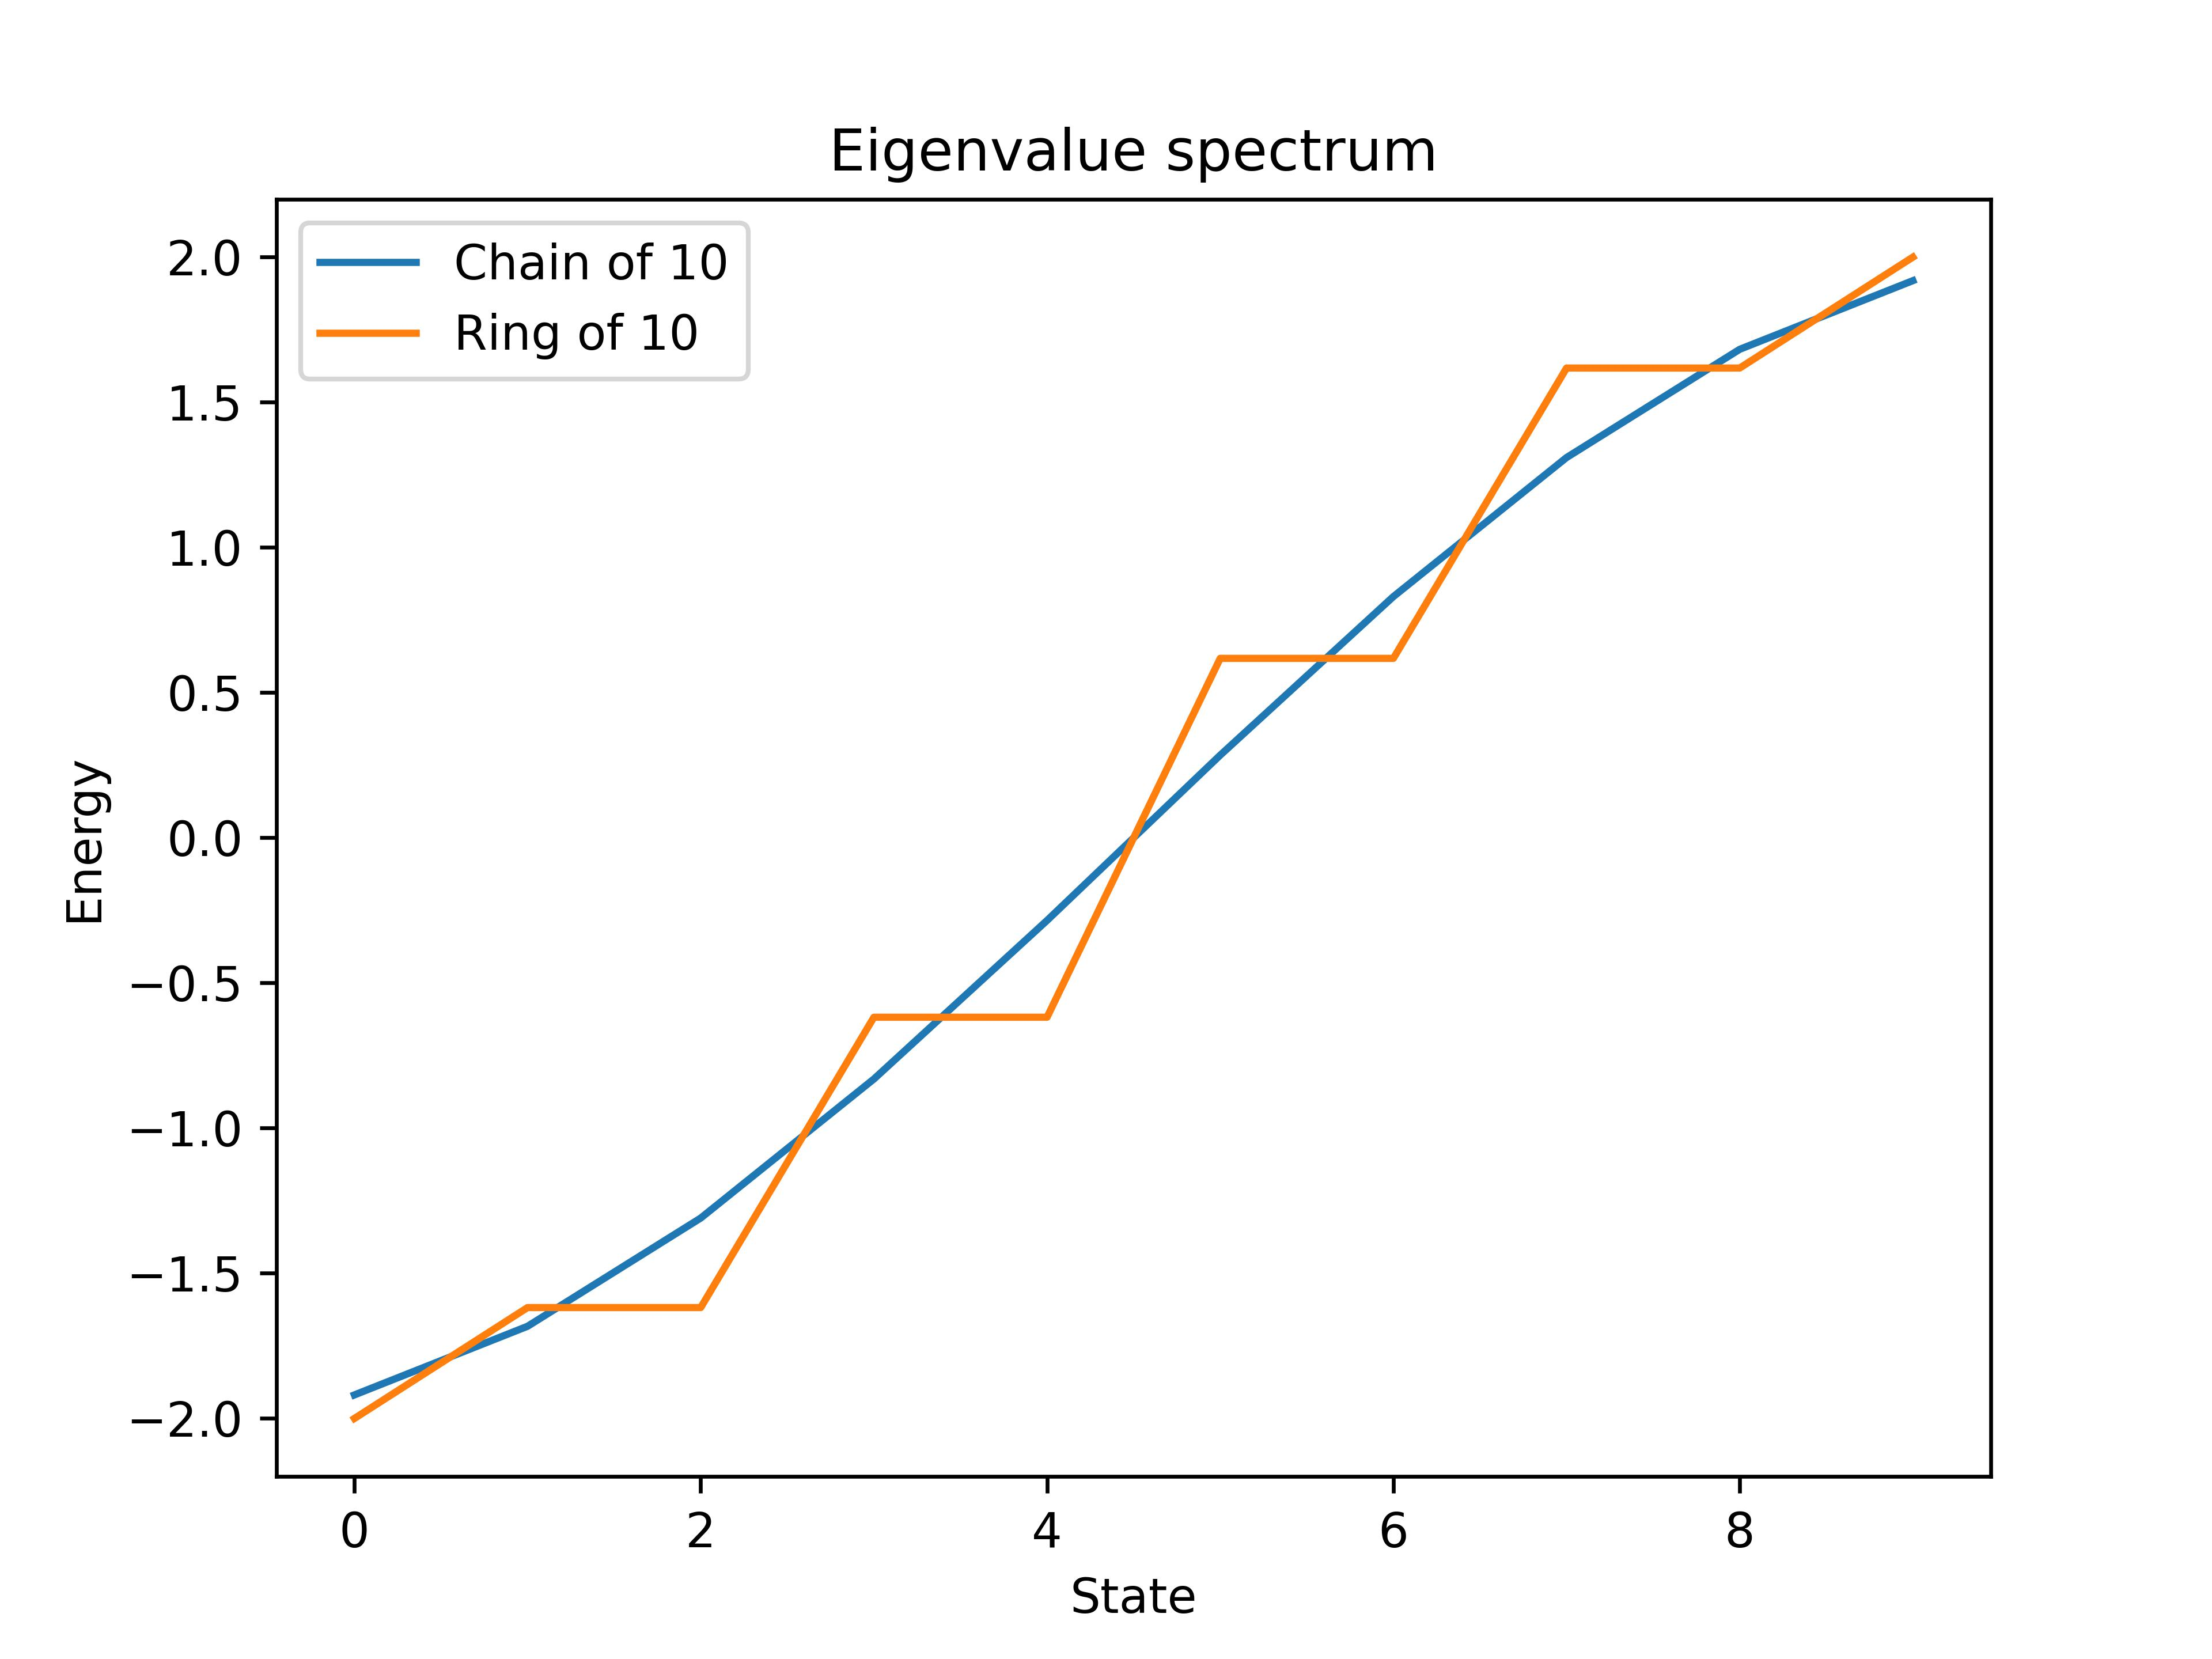
\includegraphics[width=0.75\textwidth]{Figures/chain_vs_ring.jpg}
    \caption{Comparison of eigenvalues for a chain and a ring of 10 atoms.}
    \label{fig:chain_ring}
\end{figure}

It is possible to appreciate also a big difference in the eigenvector spectrum. The eigenvectors of the first states are shown in Figures \ref{fig:chain_eigenvectors} and \ref{fig:ring_eigenvectors}. There is a notable difference between both cases. While the wave function of the ground state is localized in the central atoms in the chain as in the particle in a box, the wave function of the ring is delocalized over all the atoms. This is a consequence of the periodic boundary conditions of the ring introduced in the Hückel Hamiltonian.


\begin{figure}[h]
    \centering
    \begin{minipage}{0.45\textwidth}
        \centering
        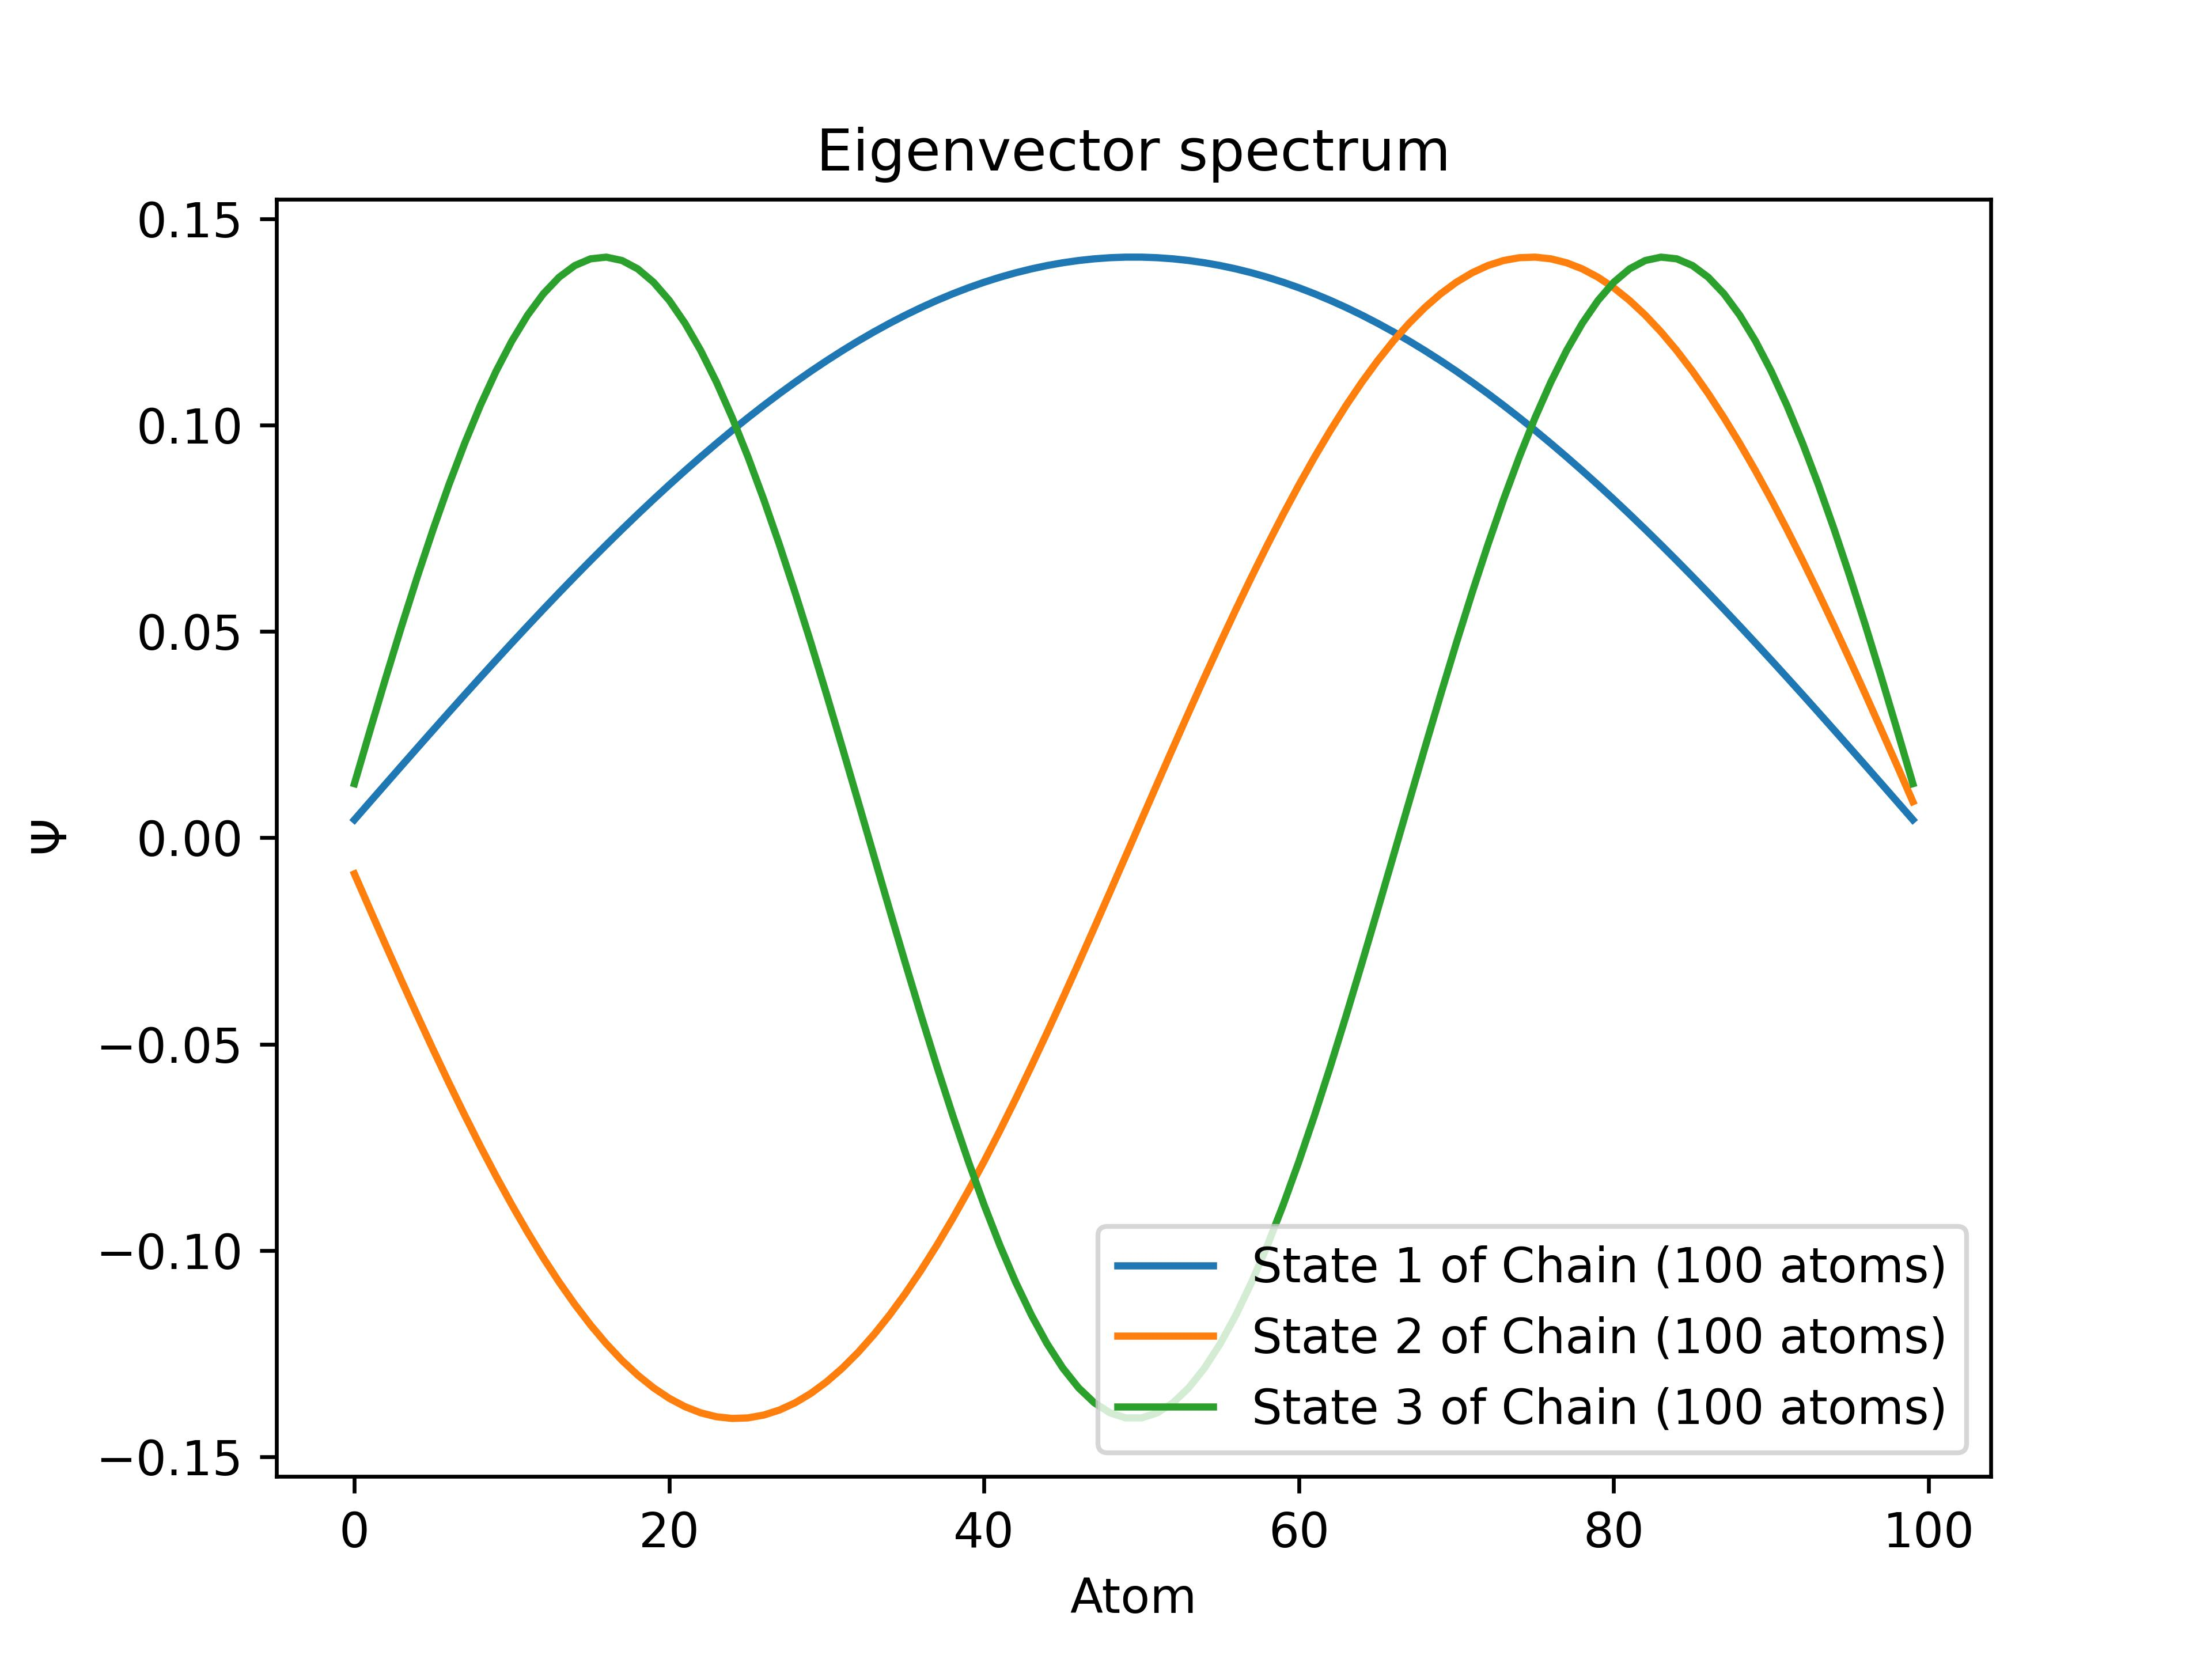
\includegraphics[width=\textwidth]{Figures/chain_eigenvectors.jpg}
        \caption{Eigenvectors for a chain of 10 atoms.}
        \label{fig:chain_eigenvectors}
    \end{minipage}
    \hfill
    \begin{minipage}{0.45\textwidth}
        \centering
        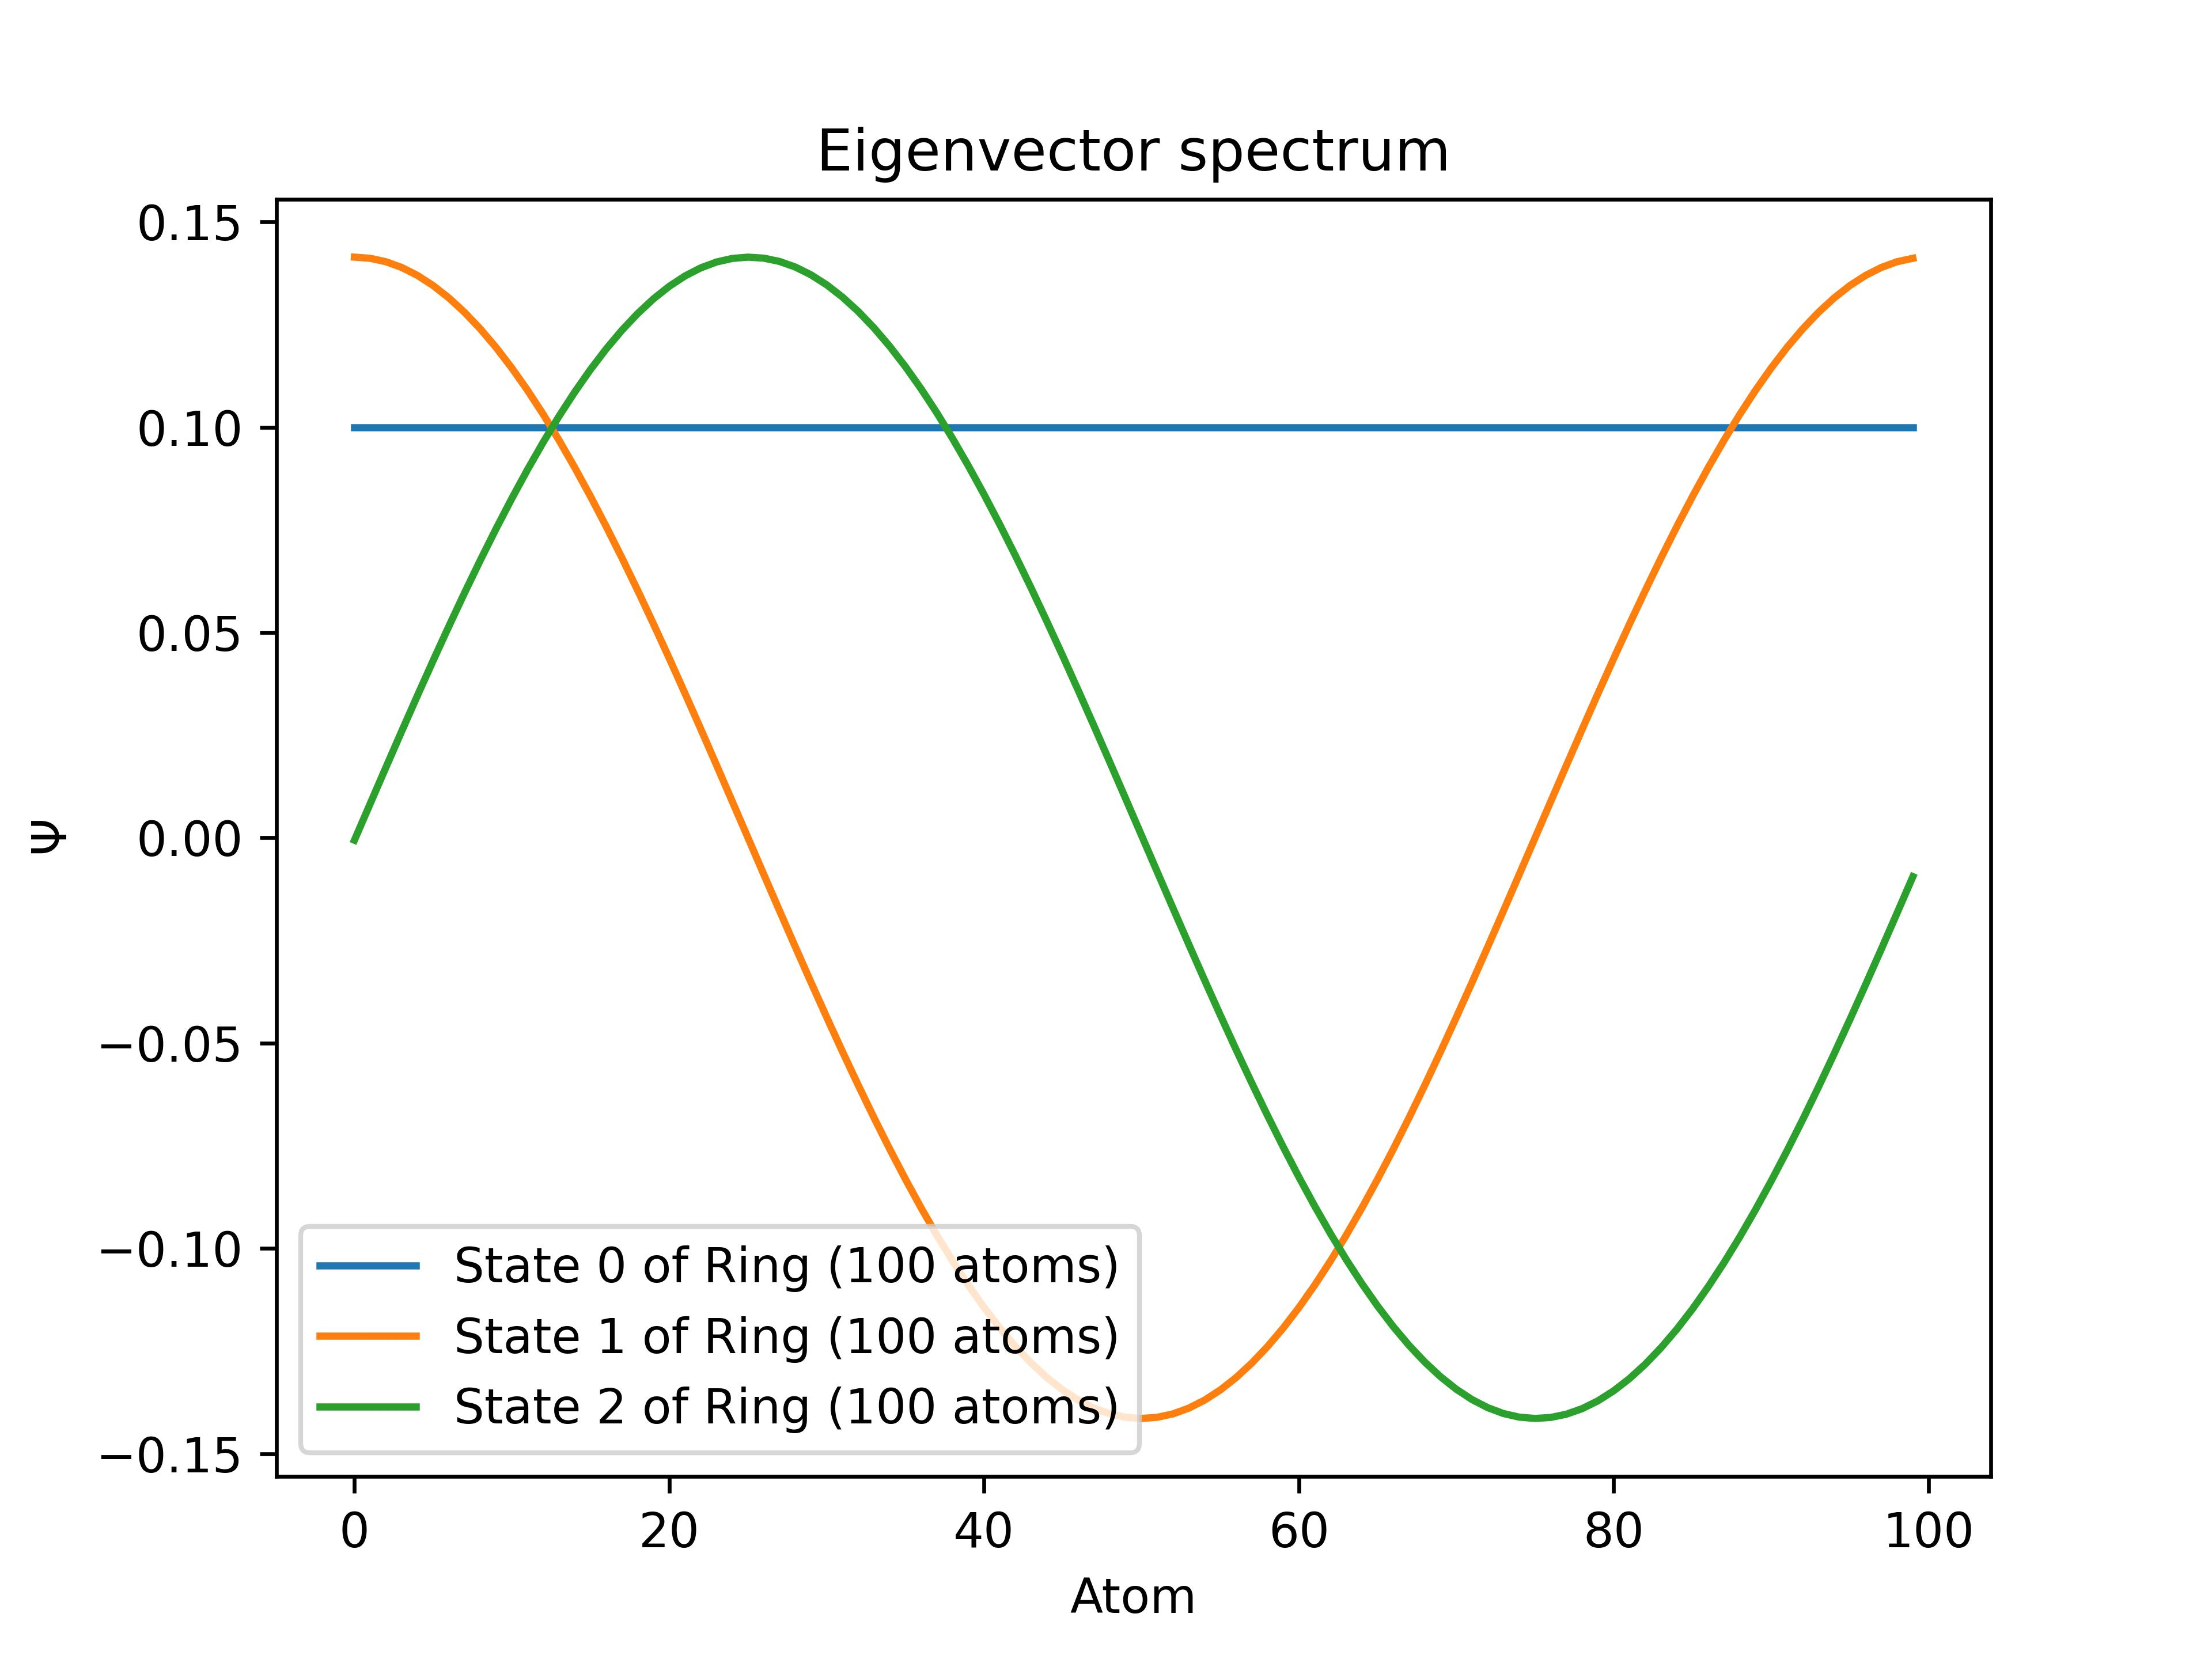
\includegraphics[width=\textwidth]{Figures/ring_eigenvectors.jpg}
        \caption{Eigenvectors for a ring of 10 atoms.}
        \label{fig:ring_eigenvectors}
    \end{minipage}
\end{figure}

It is also possible to determine that int the infinite chain limit the energy of the states converges to the energy of the ring. This is shown in Figure \ref{fig:chain_vs_ring_infinite}.

\begin{figure}[h]
    \centering
    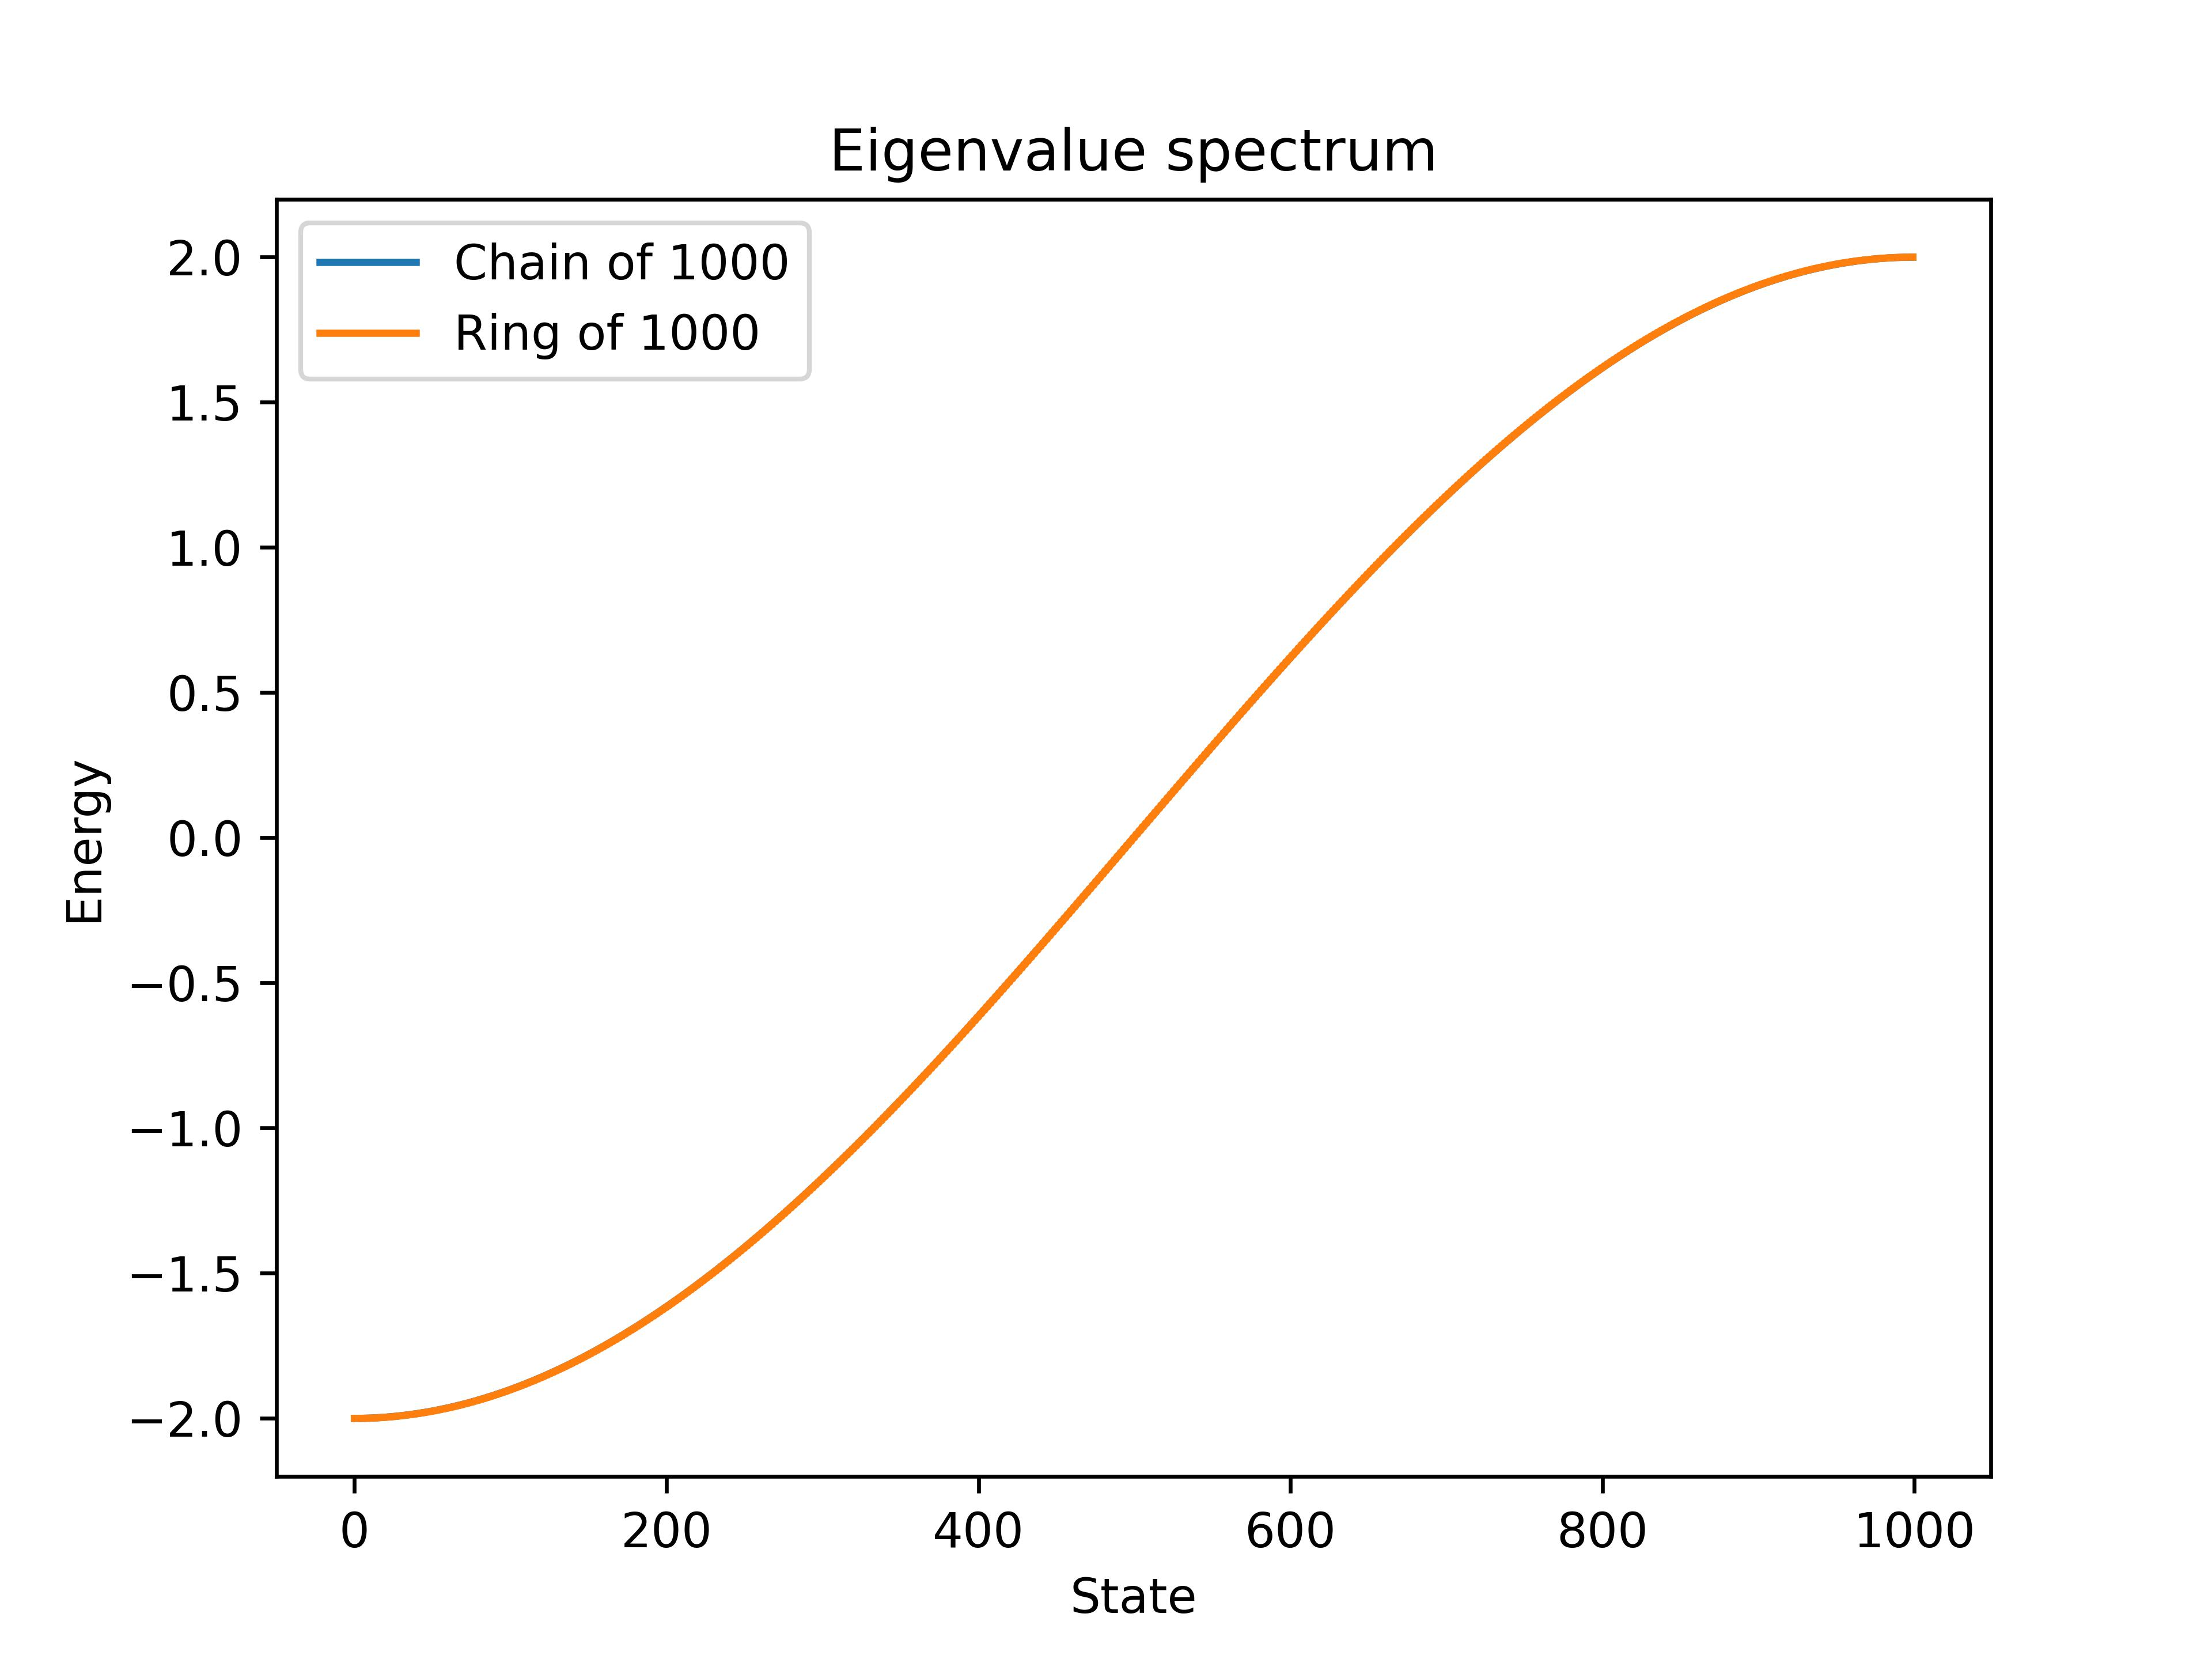
\includegraphics[width=0.75\textwidth]{Figures/convergence_limit.jpg}
    \caption{Comparison of eigenvalues for a chain and a ring of 100 atoms.}
    \label{fig:chain_vs_ring_infinite}
\end{figure}

\subsection{Alternating atoms and distances}




\begin{figure}[h]
    \centering
    \begin{minipage}{0.45\textwidth}
        \centering
        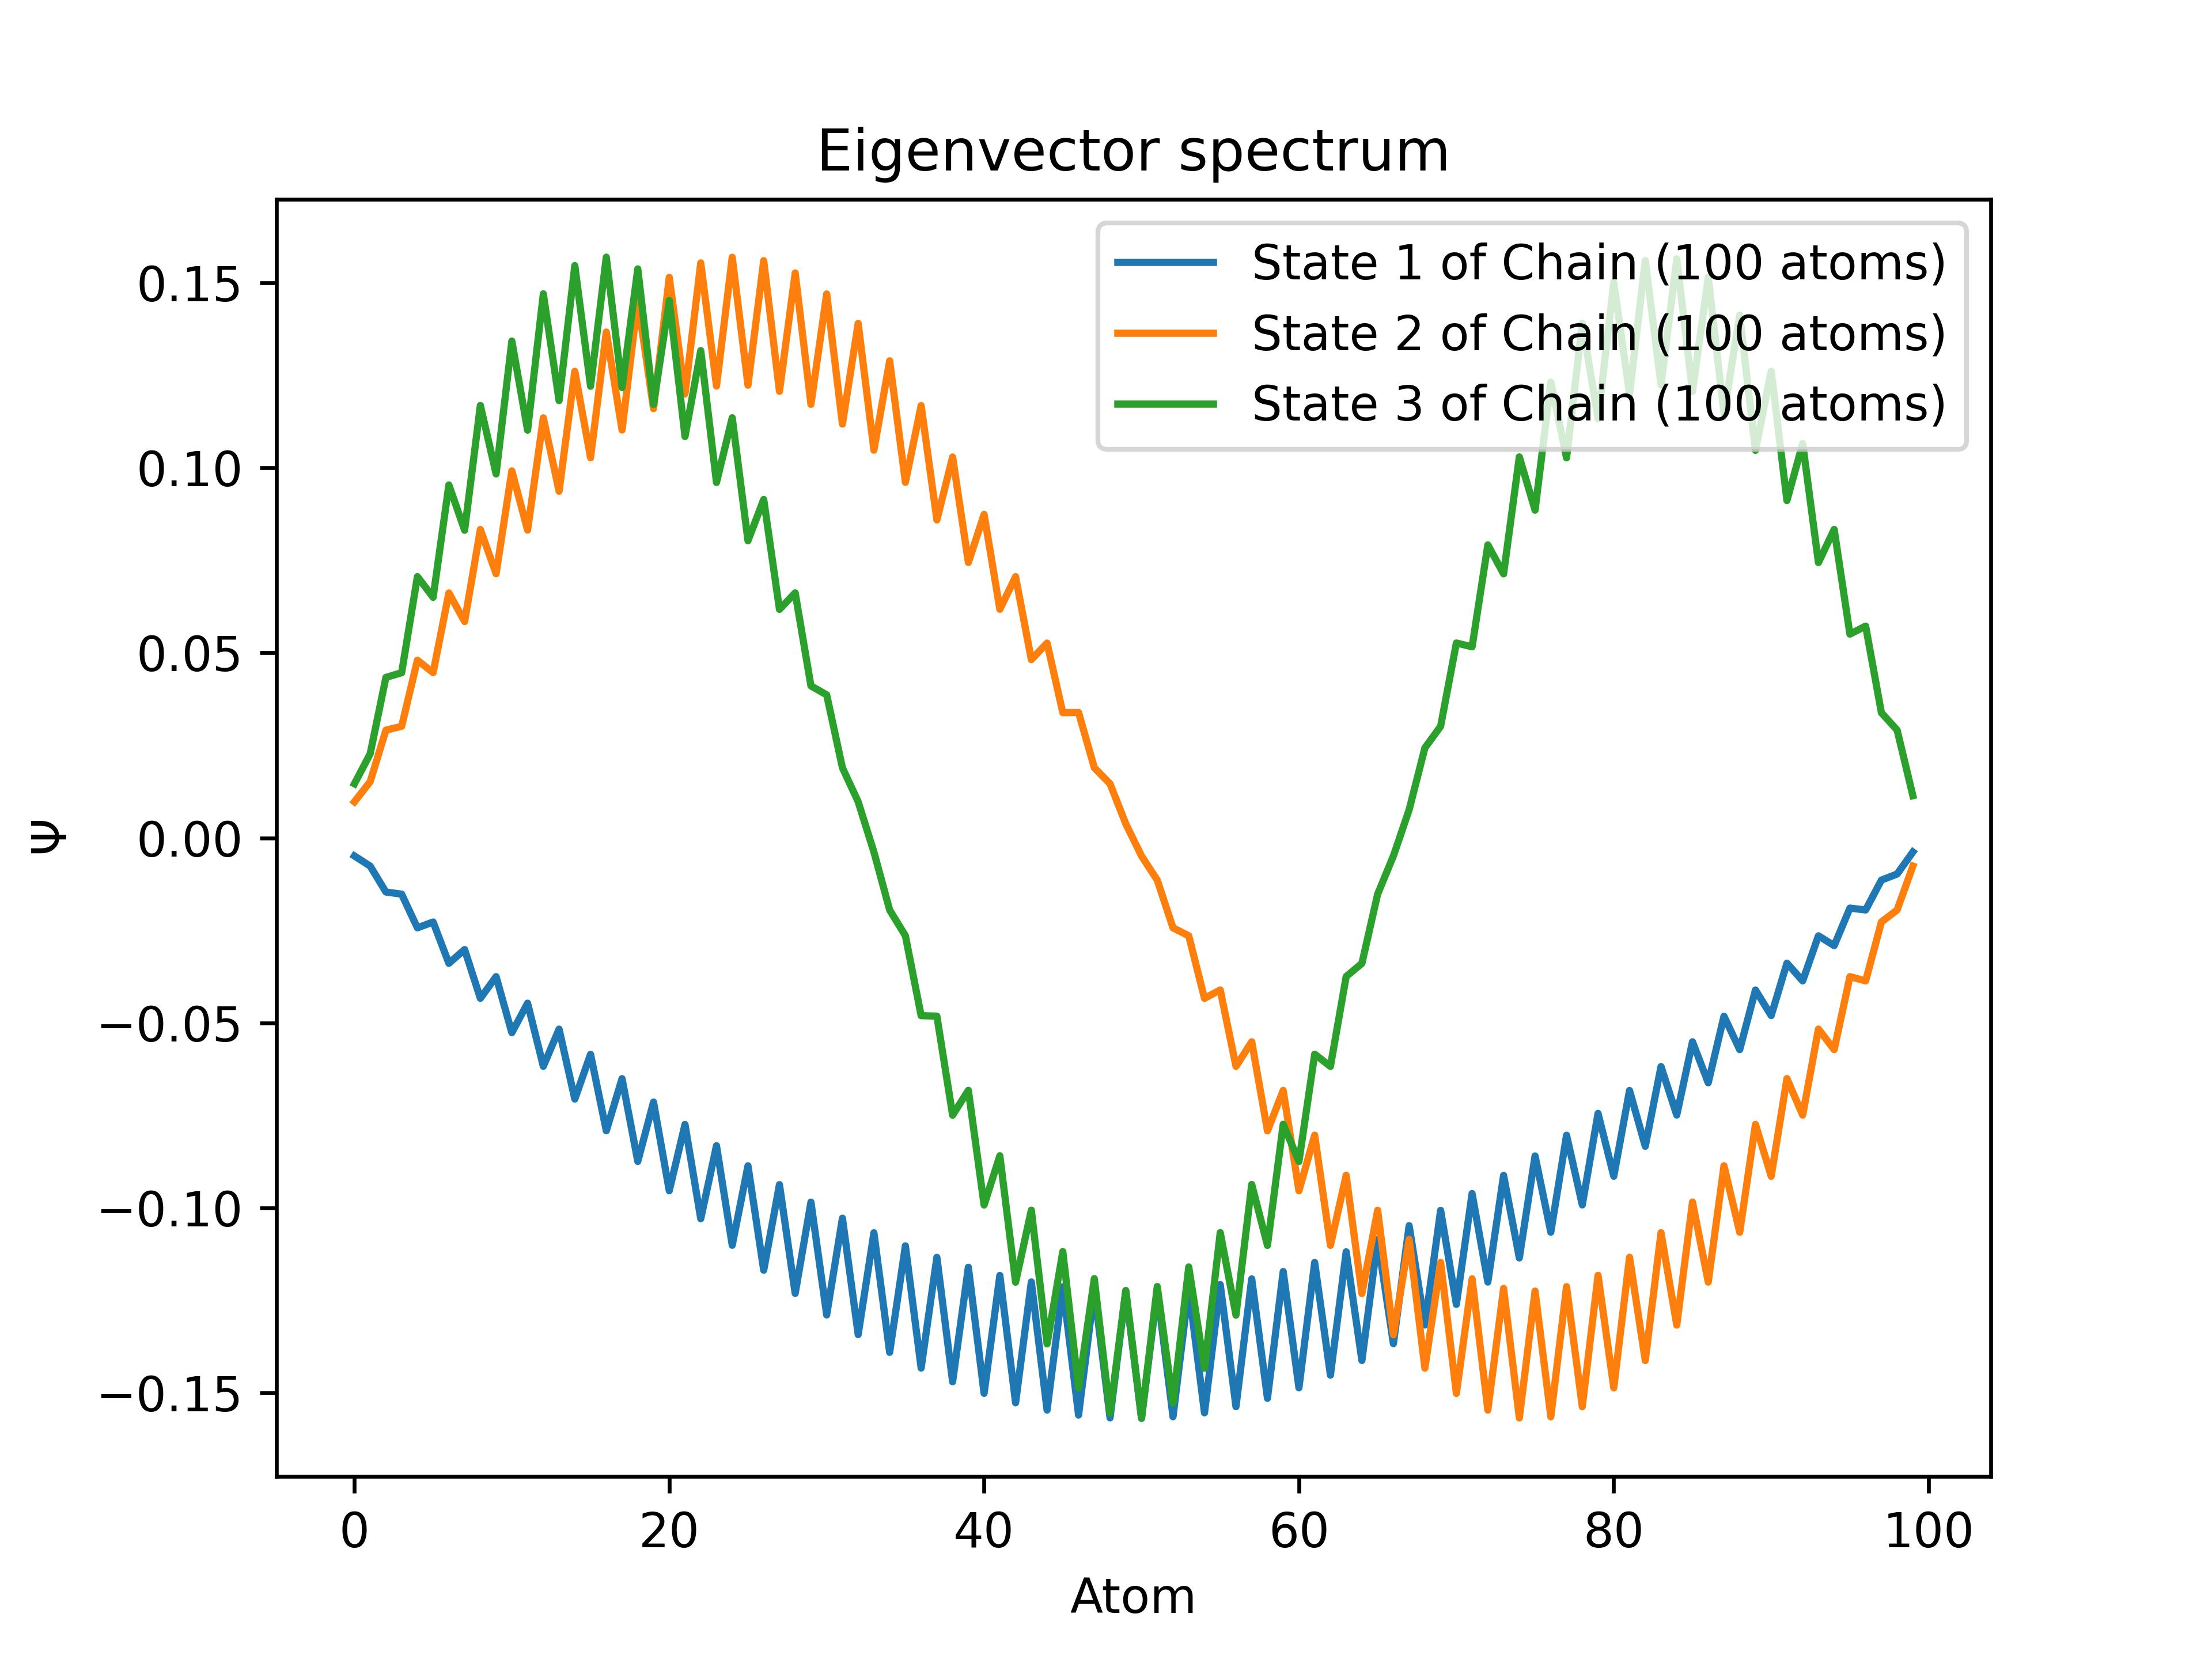
\includegraphics[width=\textwidth]{Figures/chain_alpha_eigenvectors.jpg}
        \caption{Eigenvectors for a chain with alternating $\alpha$ values.}
        \label{fig:chain_alpha_eigenvectors}
    \end{minipage}
    \hfill
    \begin{minipage}{0.45\textwidth}
        \centering
        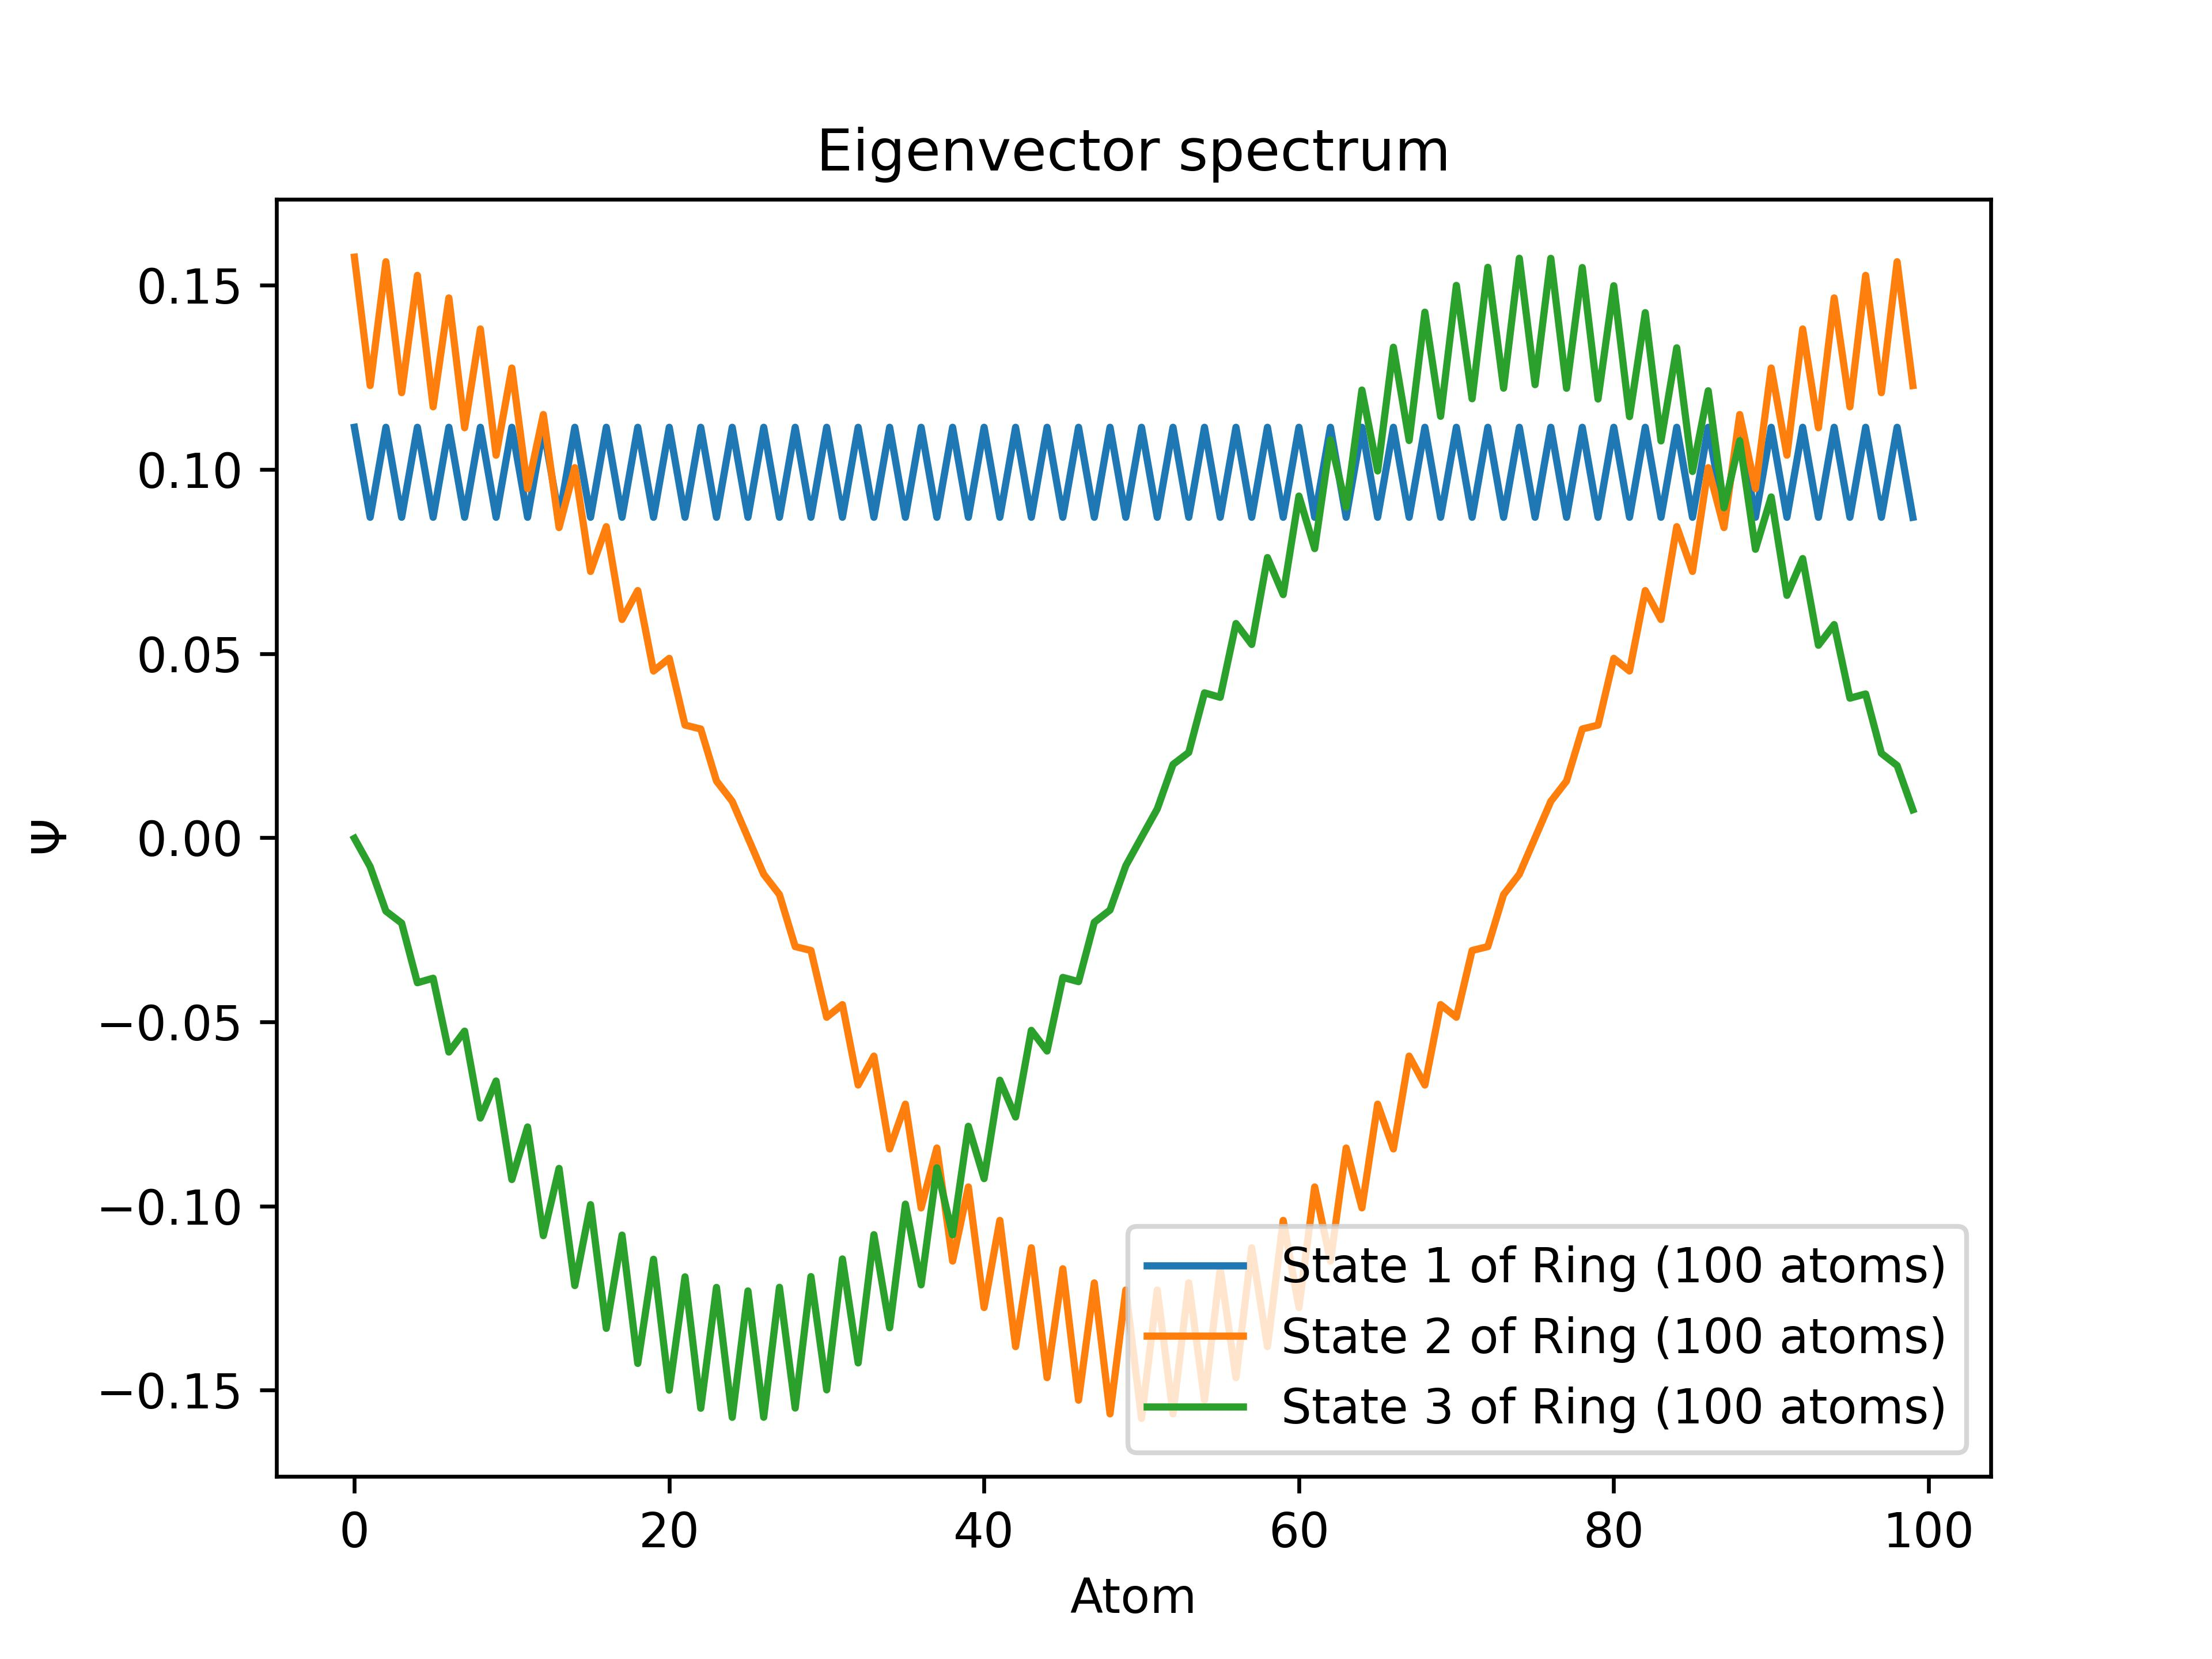
\includegraphics[width=\textwidth]{Figures/ring_alpha_eigenvectors.jpg}
        \caption{Eigenvectors for a ring with alternating $\alpha$ values.}
        \label{fig:ring_alpha_eigenvectors}
    \end{minipage}
\end{figure}


\begin{figure}[h]
    \centering
    \begin{minipage}{0.45\textwidth}
        \centering
        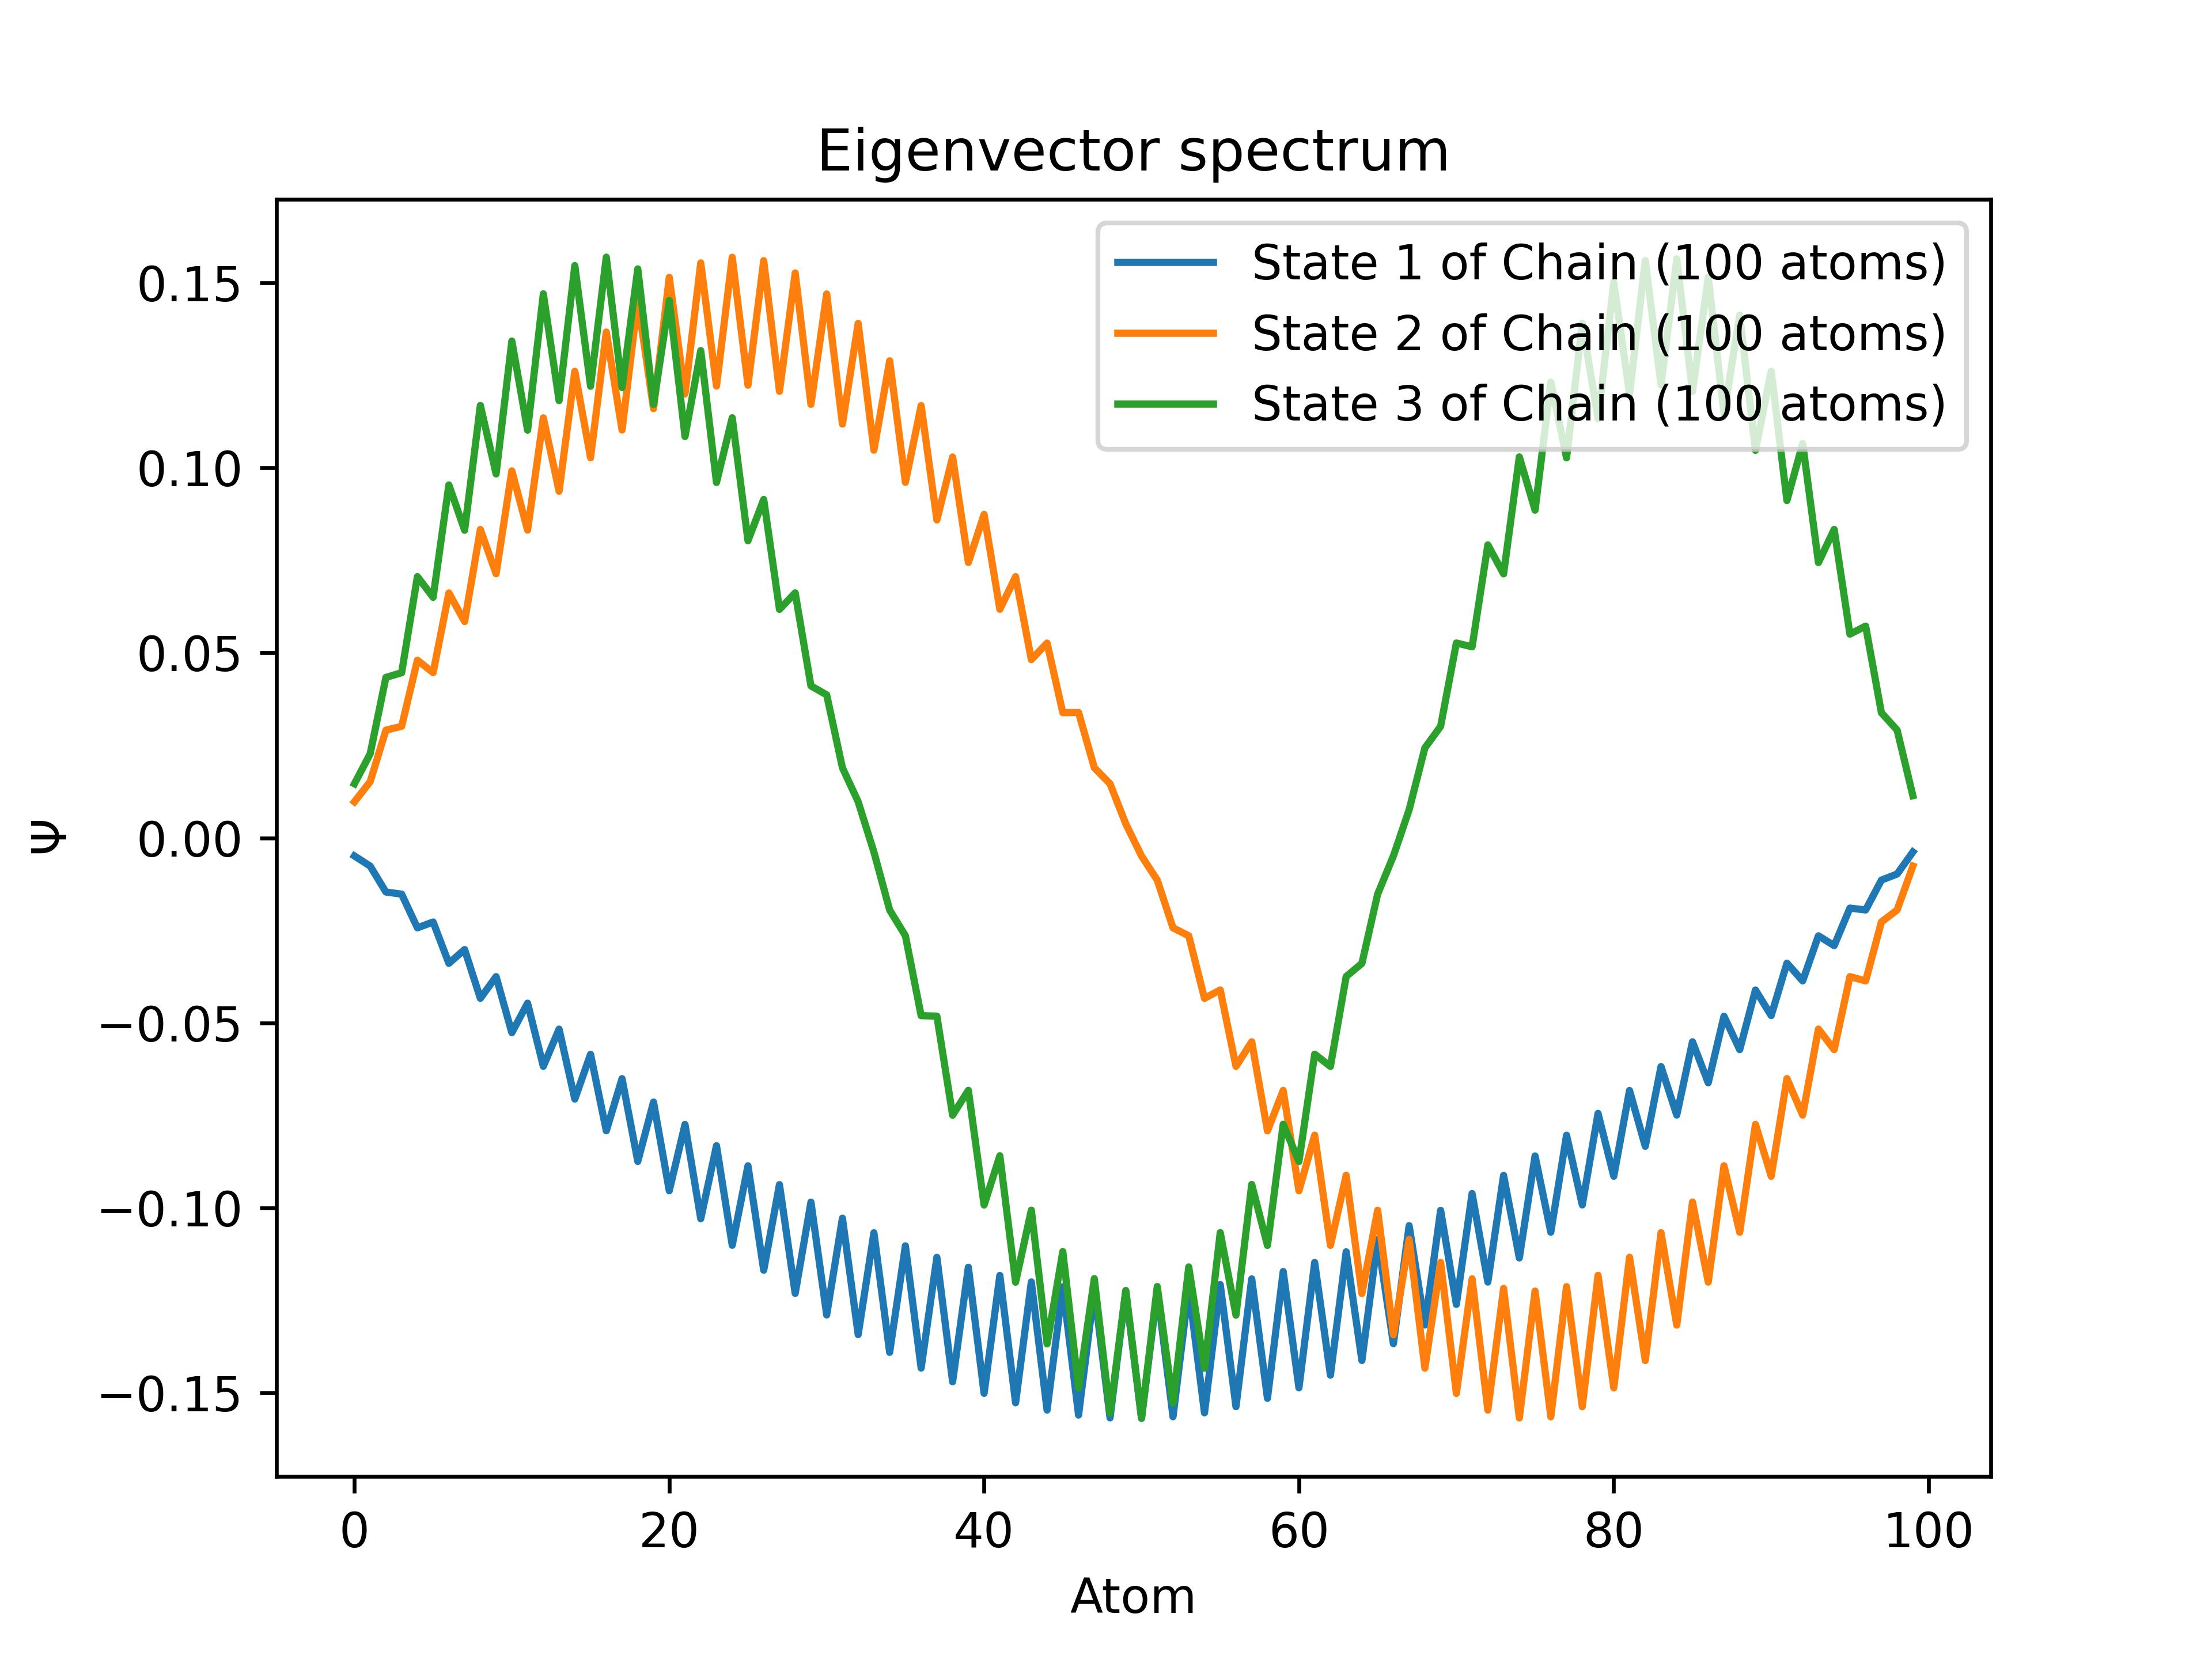
\includegraphics[width=\textwidth]{Figures/chain_alpha_eigenvectors.jpg}
        \caption{Eigenvectors for a chain with alternating $\alpha$ values.}
        \label{fig:chain_alpha_eigenvectors}
    \end{minipage}
    \hfill
    \begin{minipage}{0.45\textwidth}
        \centering
        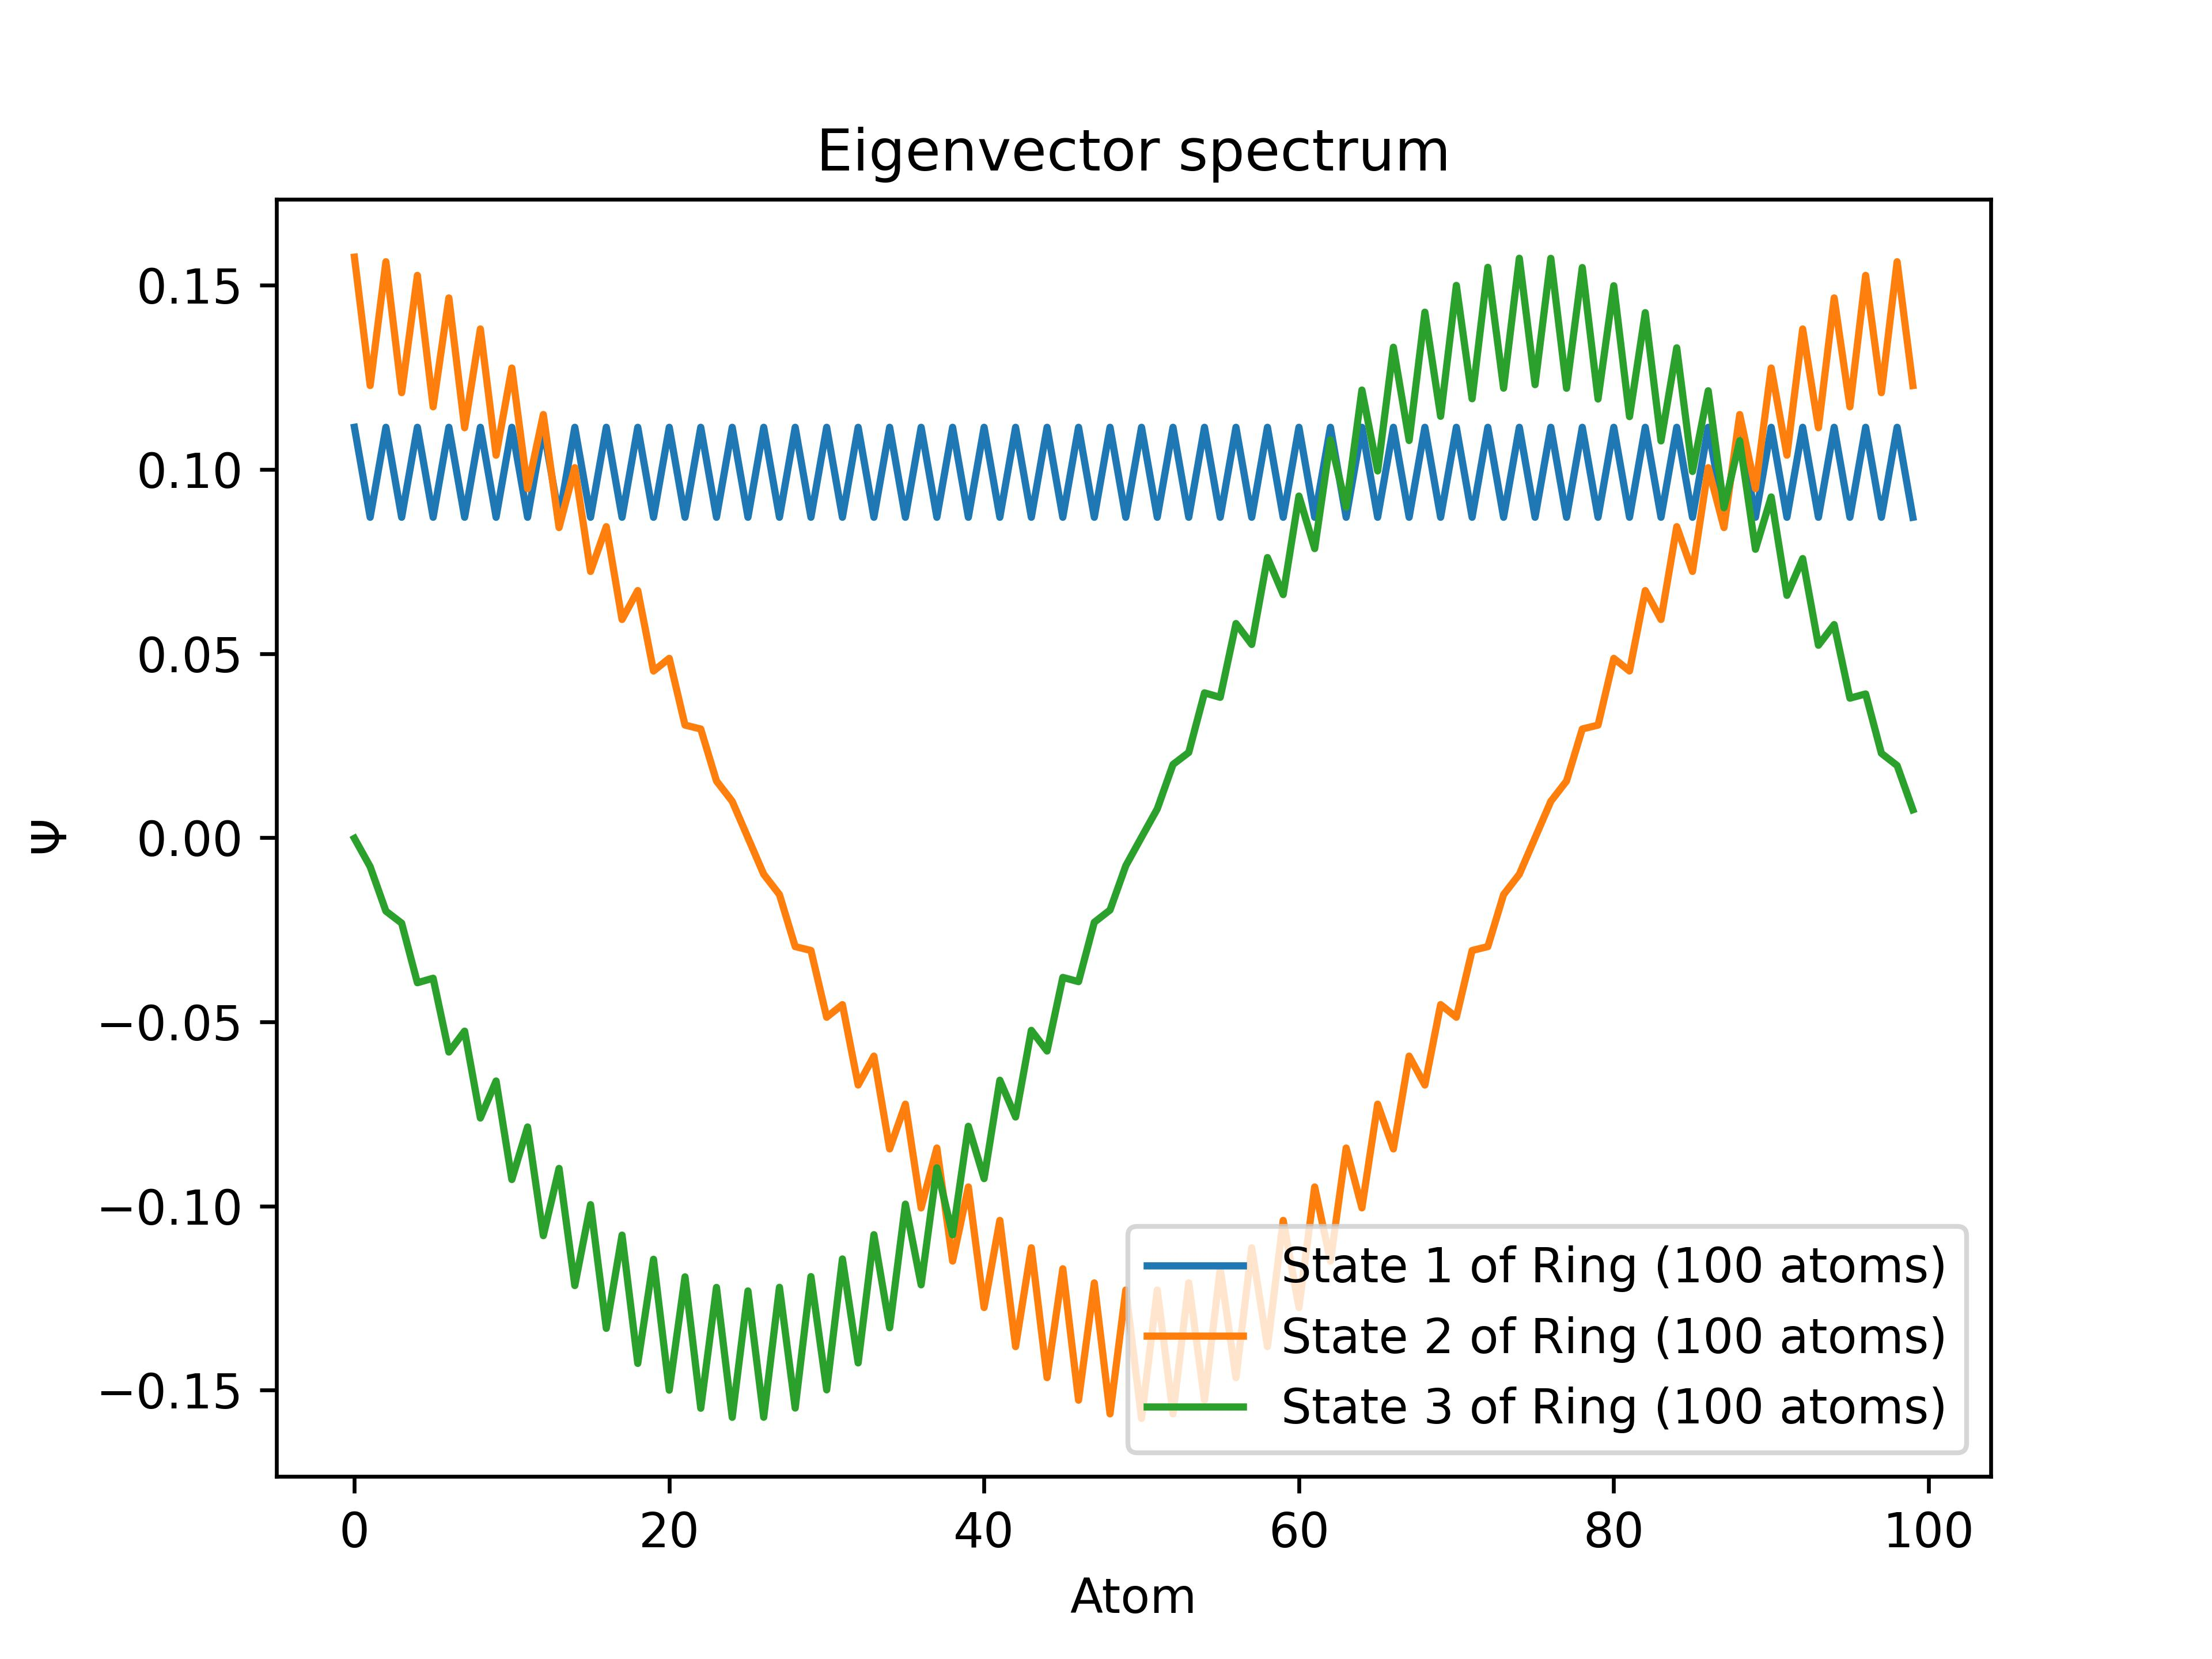
\includegraphics[width=\textwidth]{Figures/ring_alpha_eigenvectors.jpg}
        \caption{Eigenvectors for a ring with alternating $\alpha$ values.}
        \label{fig:ring_alpha_eigenvectors}
    \end{minipage}
    \vfill
    \begin{minipage}{0.45\textwidth}
        \centering
        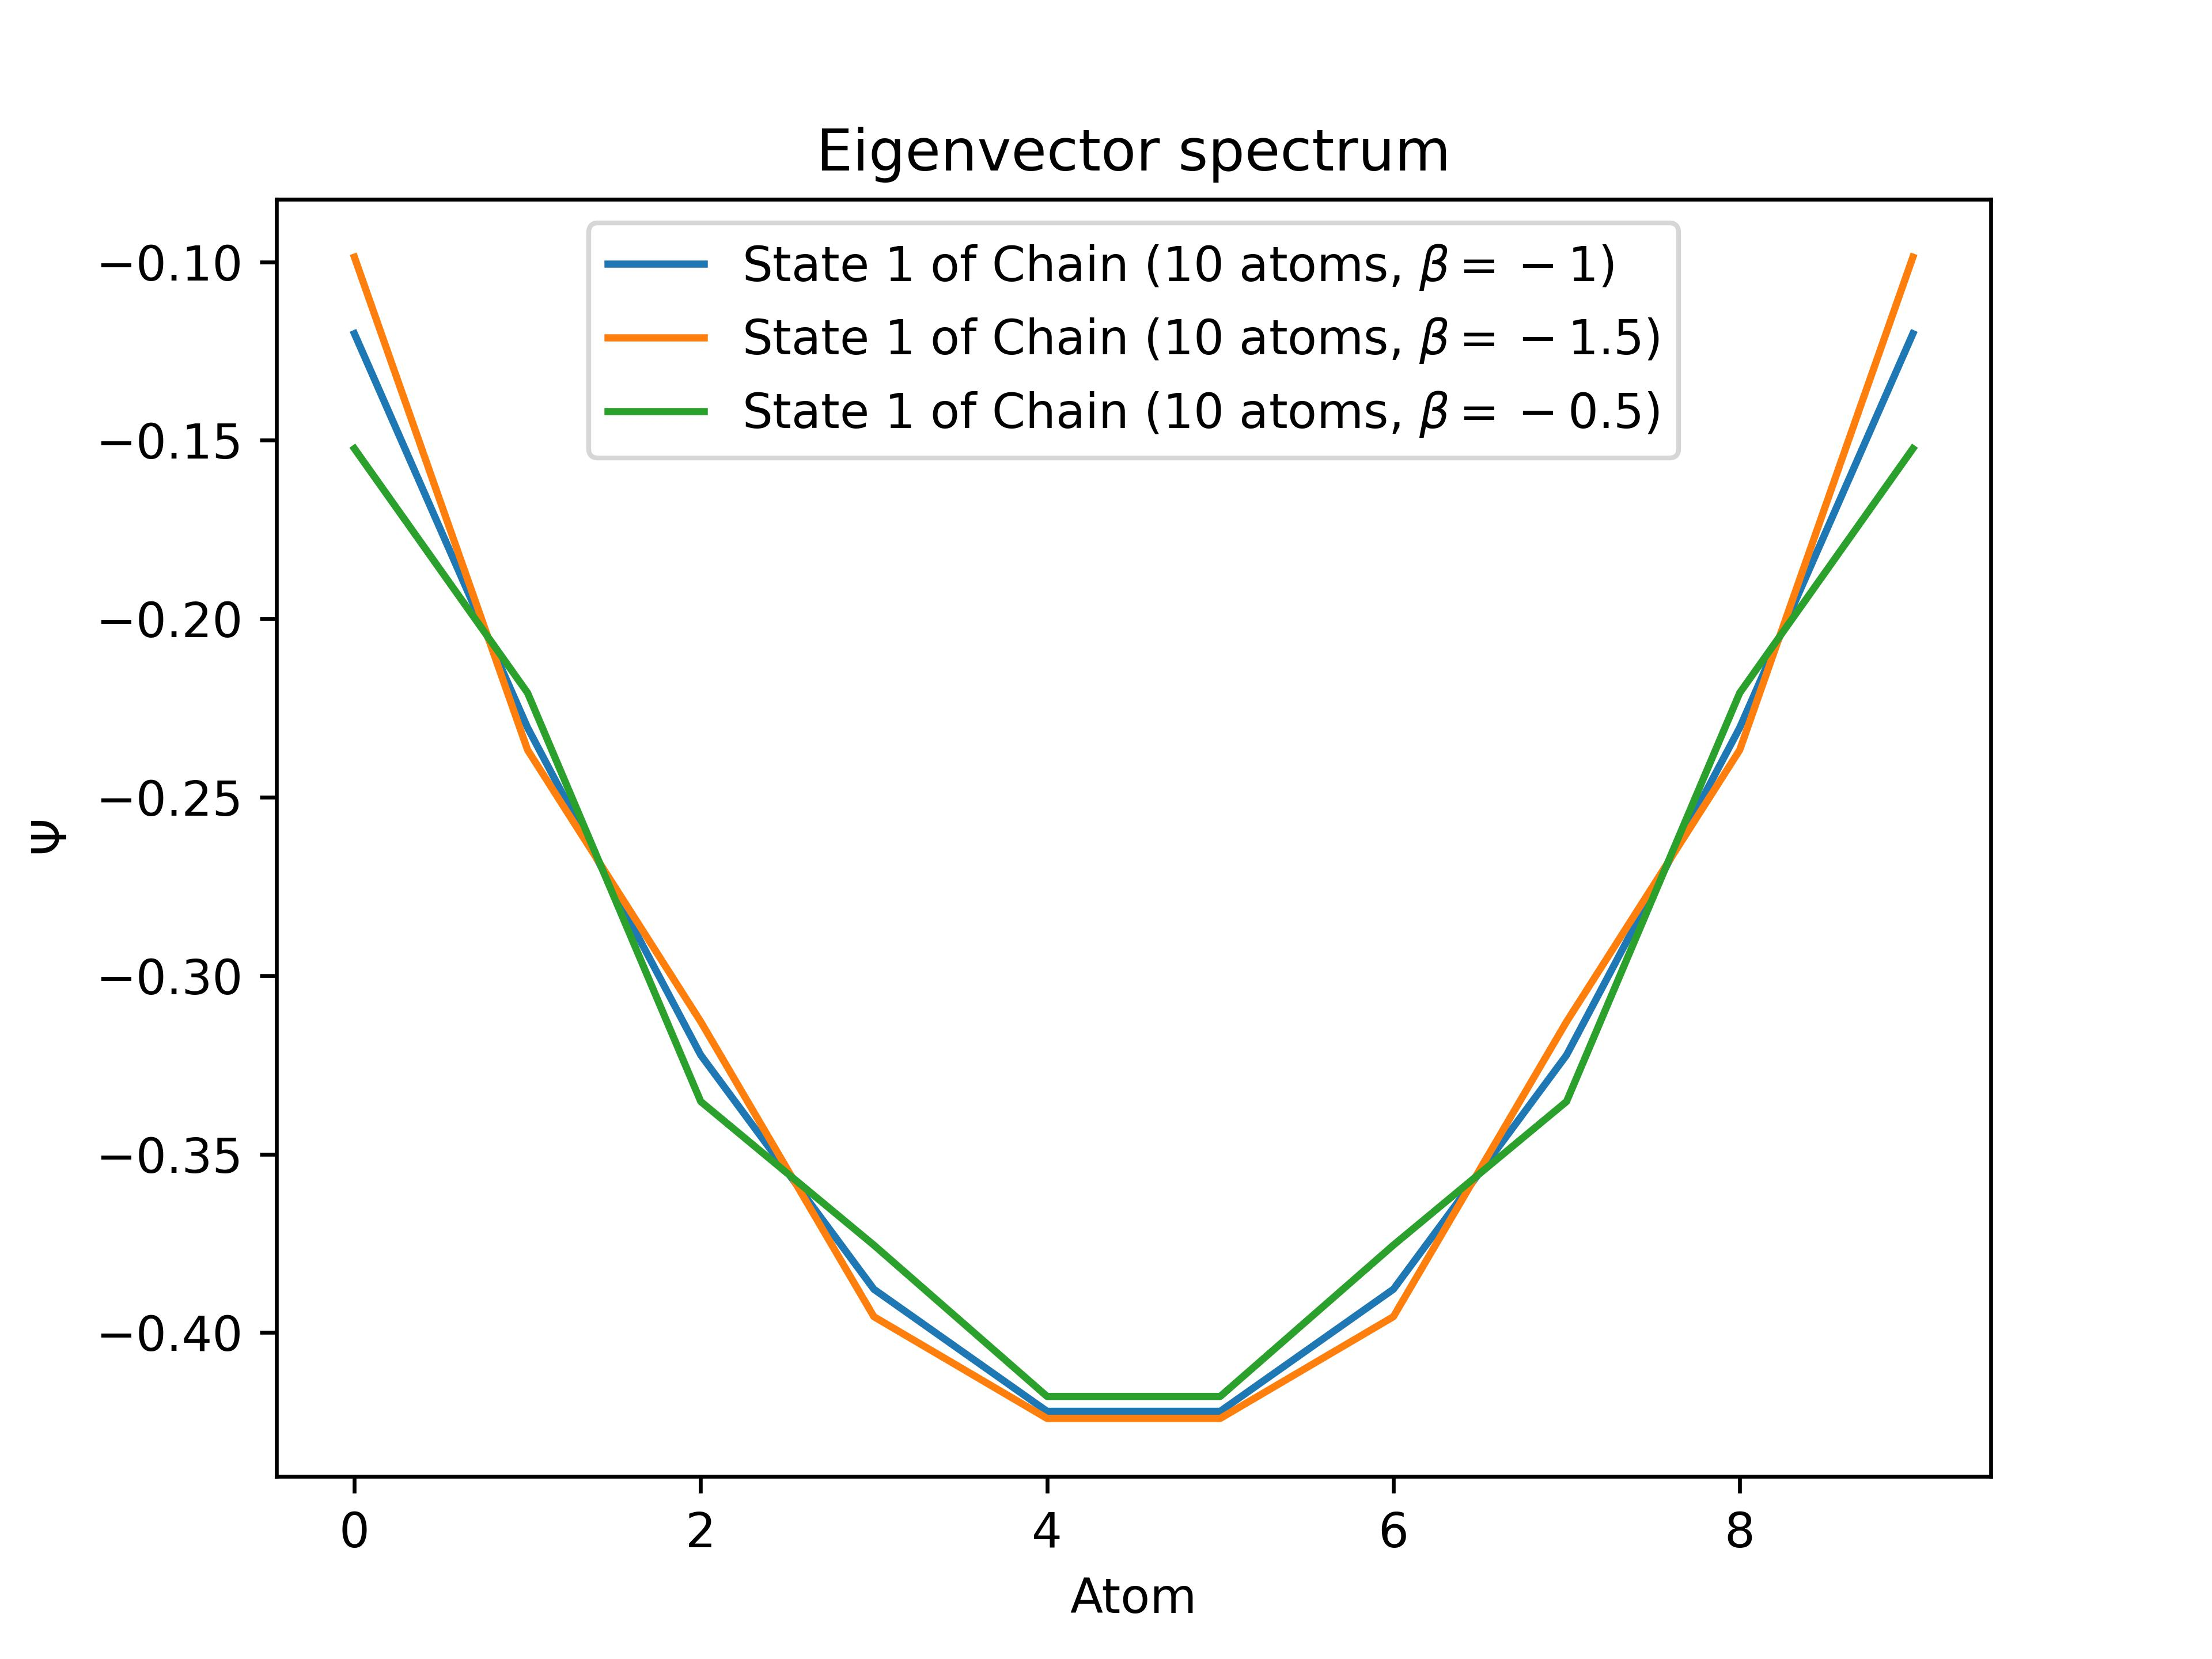
\includegraphics[width=\textwidth]{Figures/chain_beta_eigenvectors.jpg}
        \caption{Eigenvectors for a chain with alternating $\beta$ values.}
        \label{fig:chain_beta_eigenvectors}
    \end{minipage}
    \hfill
    \begin{minipage}{0.45\textwidth}
        \centering
        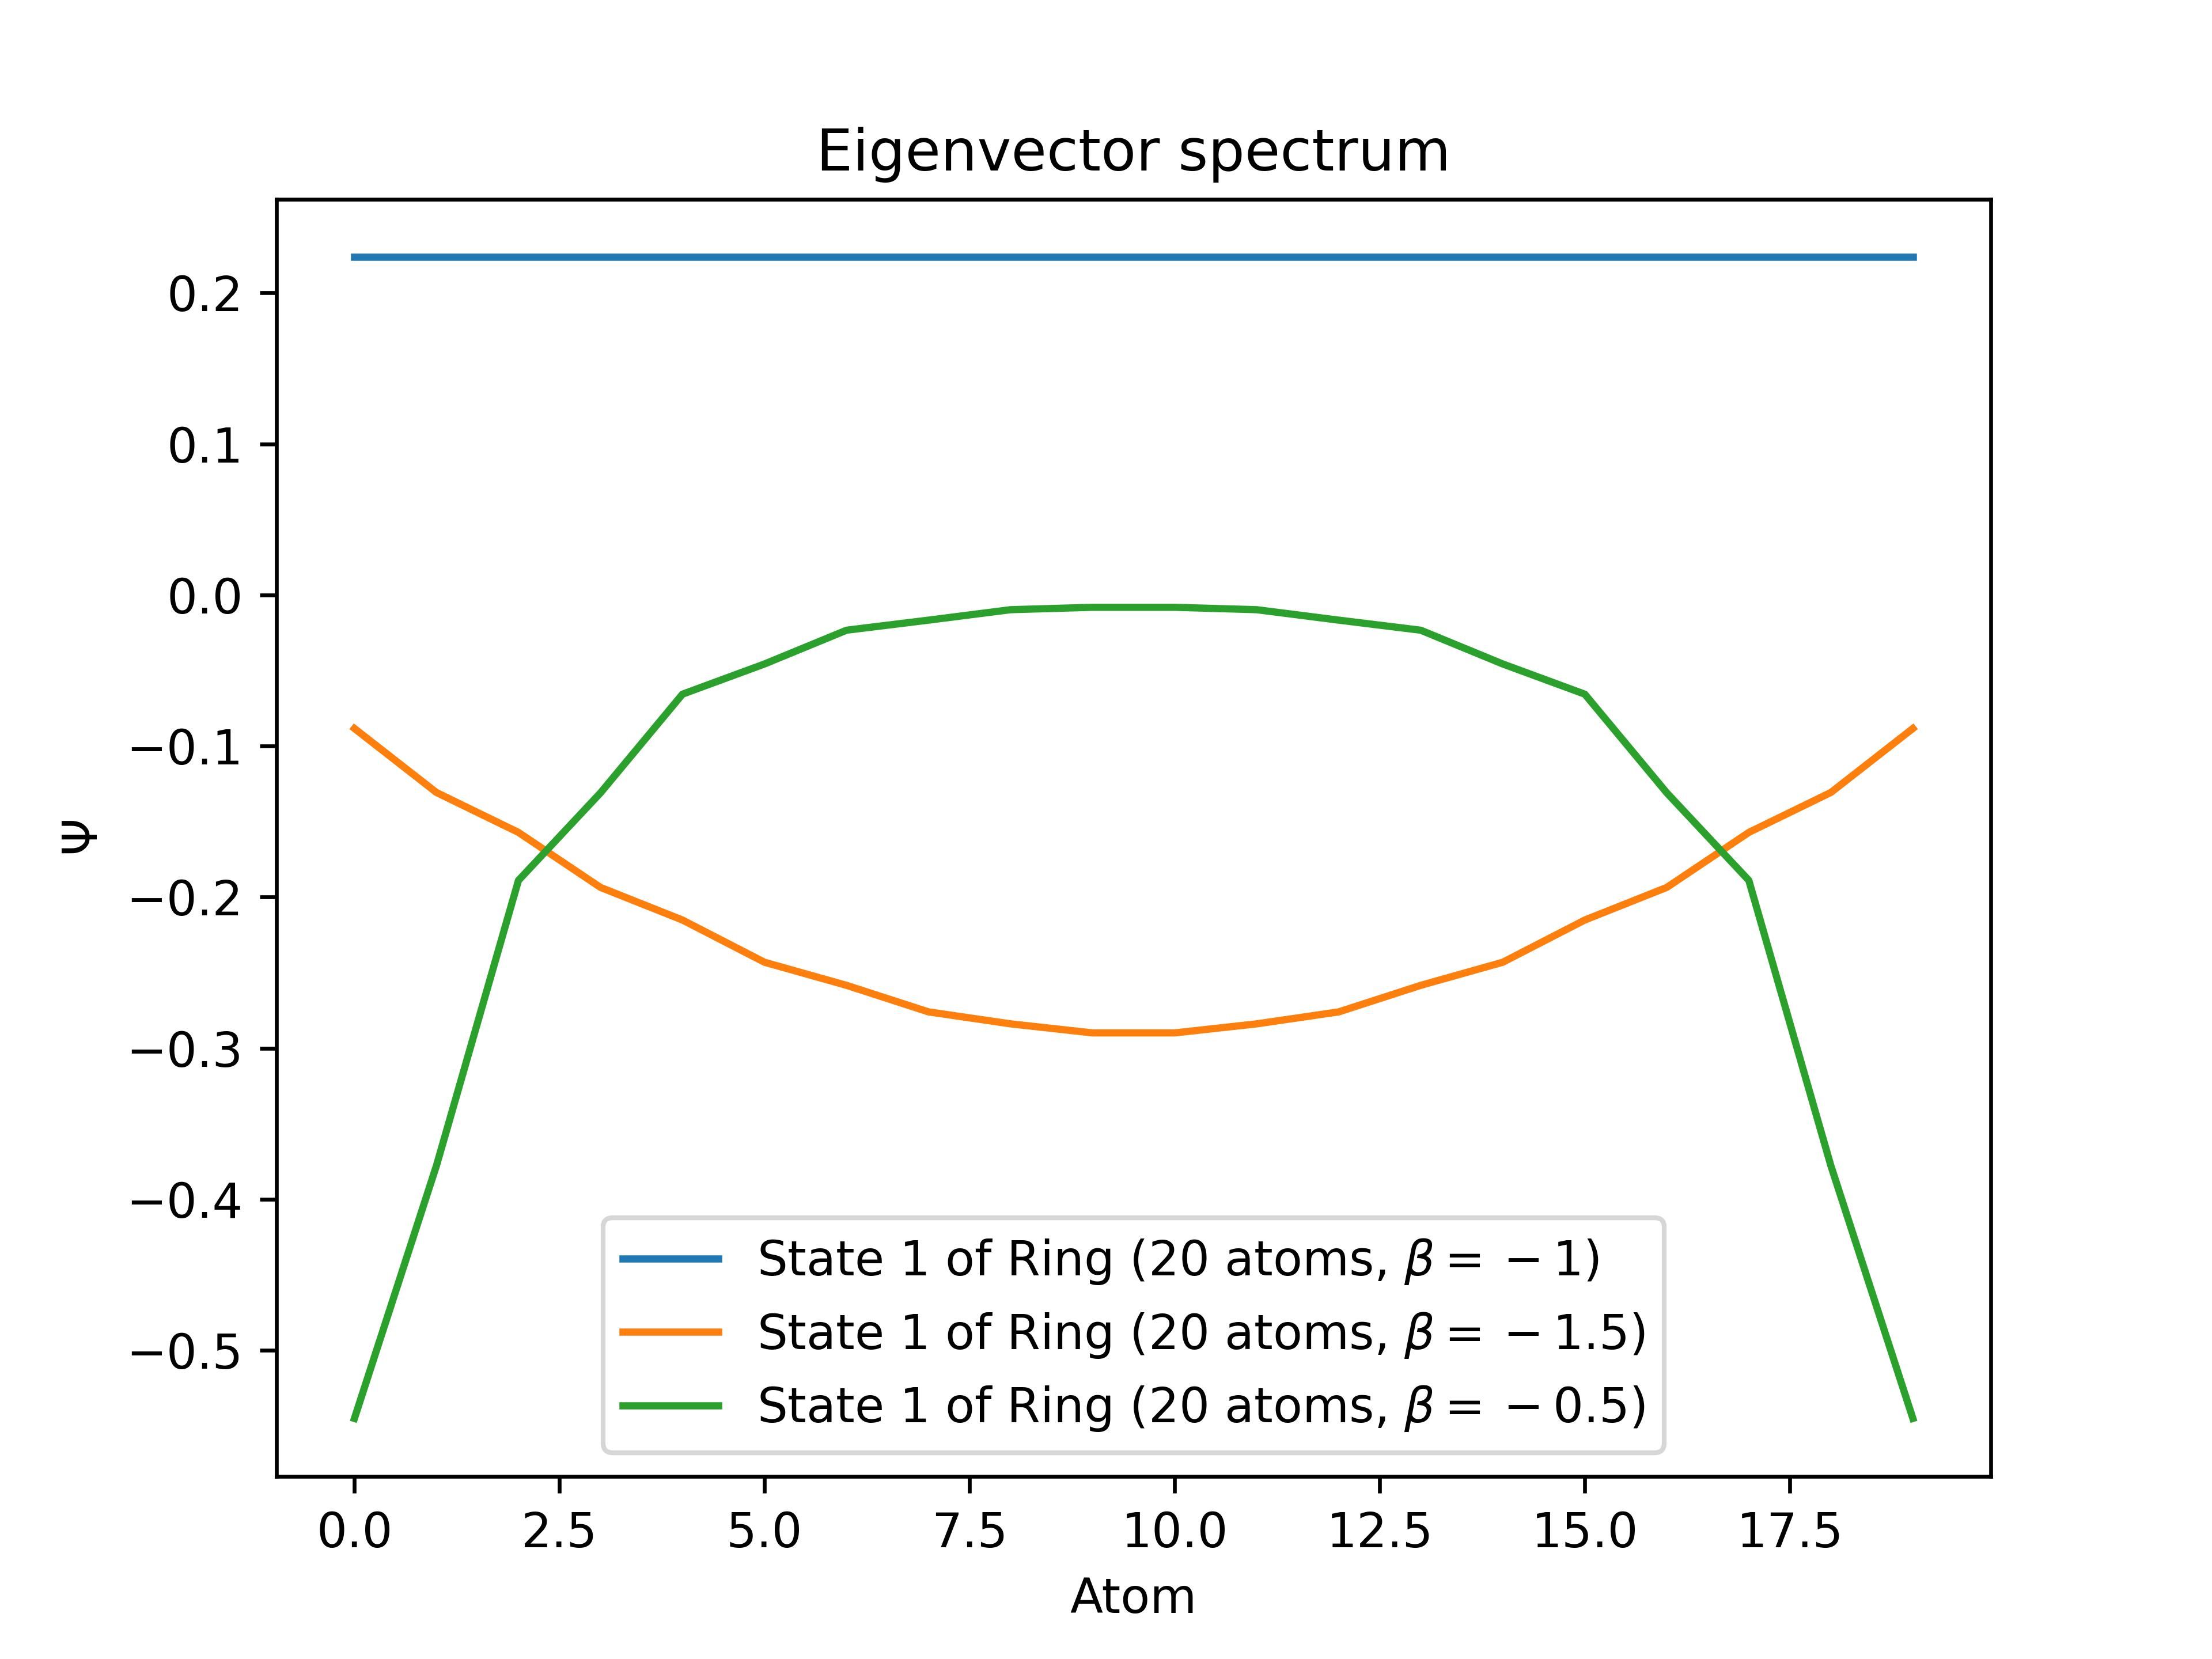
\includegraphics[width=\textwidth]{Figures/ring_beta_eigenvectors.jpg}
        \caption{Eigenvectors for a ring with alternating $\beta$ values.}
        \label{fig:ring_beta_eigenvectors}
    \end{minipage}
\end{figure}

% \printbibliography

\end{document}
